% AER-Article.tex for AEA last revised 22 June 2011
\documentclass[pdftex]{article}

\RequirePackage[OT1]{fontenc}

\RequirePackage{graphicx}
\RequirePackage{amsthm}
%\RequirePackage{amsmath}
\RequirePackage{natbib}
%\RequirePackage[colorlinks,citecolor=blue,urlcolor=blue]{hyperref}
%\RequirePackage{hypernat}
\RequirePackage[dvips]{color}
%\RequirePackage{breqn}
%\Requirepackage[T1]{fontenc}
\RequirePackage[latin9]{inputenc}
%\RequirePackage{enumitem}
%\RequirePackage{bbm}
\RequirePackage{amssymb}
\RequirePackage{stmaryrd}
\RequirePackage{nicefrac}
%\RequirePackage{amsfonts}
%\RequirePackage[english]{babel}
\RequirePackage{tikz}

%\RequirePackage[OT1]{fontenc}
%\RequirePackage{graphicx}
%\RequirePackage{amsthm}
\RequirePackage[cmex10]{amsmath}
%\RequirePackage{natbib}
%\RequirePackage[colorlinks,citecolor=blue,urlcolor=blue]{hyperref}
%\RequirePackage{hypernat}
\RequirePackage[dvips]{color}
%\RequirePackage{breqn}
%\Requirepackage[T1]{fontenc}
%\RequirePackage[latin9]{inputenc}
\RequirePackage{enumitem}
\RequirePackage{bbm}
%\RequirePackage{amssymb}
%\RequirePackage{stmaryrd}
%\RequirePackage{nicefrac}
\RequirePackage{amsfonts}
%\RequirePackage[english]{babel}
%\RequirePackage{tikz}
\usepackage{subcaption}
\usepackage{setspace}
\usepackage{caption}
\usepackage{authblk}
%\startlocaldefs



\numberwithin{equation}{section}
\newtheoremstyle{th}
  {\topsep}%Space above
  {\topsep}%Space below
  {\itshape}%Body font
  {}%Indent amount
  {\normalfont}% Theorem head font
  {:}%Punctuation after theorem head
  { }%Space after theorem head
  {}% Theorem head specification
\theoremstyle{th}
\newtheorem{thm}{{Theorem}}%[section]
\newtheorem{lemma}{{Lemma}.}%[section]
\newtheorem{conjecture}{{Conjecture}.}%[section]
\newtheorem{prop}{{Proposition}}%[section]
  \newtheorem{cor}{{Corollary}}%[section]%{\protect\corollaryname}
\newtheorem{proof lemma}{{Proof Lemma}.}
\theoremstyle{definition}
\newtheorem{A}{A\hspace{-0.15cm}}
\newtheorem{B}{B\hspace{-0.15cm}}
\newtheorem*{TK}{TK\hspace{-0.15cm}}
\newtheorem*{JS}{JS\hspace{-0.15cm}}
\newtheorem{SA}{SA\hspace{-0.15cm}}
\newtheorem{ceu}{CEU\hspace{-0.15cm}}
\newtheorem{definition}{Definition}%[section]
\newtheorem{example}{Example}%[section]
\newtheorem{remark}{Remark}%[section]
\newtheorem{statement}{Statement.}%[section]
\newtheorem{fact}{Fact}%[section]



%\Spacing{2}

\begin{document}

\title{General equilibrium with uncertainty loving preferences}
\author[1,2]{A. Araujo\thanks{We thank participants at the 10th Annual Cowles GE 2014 Conference, the 13th SAET 2013 Conference, EEA-ESEM 2014, IWGTS 2014, EWGET 2014, LACEA-LAMES 2014, the 15th SAET 2015 Conference and the 11th World Congress of the Econometric Society for comments. We also thank T. Kehoe, P.A. Chiappori, P. Wakker, T. Strzalecki, C. Azariadis and Braulio Calagua and all the anonymous referees for their comments and suggestions that improved our work. The authors gratefully acknowledge financial support from CAPES, CNPq and FAPERJ, Chateauneuf and Gama thank IMPA for the generous financial support from the ``Ci\^{e}ncias sem Fronteiras'' fellowship and from the ``Brazilian$-$French Network in Mathematics''.}\thanks{aloisio@impa.br}}
\author[3]{A. Chateauneuf\thanks{Alain.Chateauneuf@univ-paris1.fr}}
\author[1]{J. Gama\thanks{jpgamat@impa.br}}
\author[4]{R. Novinski\thanks{rodrigo.novinski@ibmecrj.br}}
\affil[1]{IMPA, Rio de Janeiro, Brazil}
\affil[2]{EPGE/FGV, Rio de Janeiro, Brazil}
\affil[3]{IPAG Business School and Paris School of Economics, Universit\'{e} de Paris I, Paris, France}
\affil[4]{Faculdades Ibmec-RJ, Rio de Janeiro, Brazil}

\date{\today}
\maketitle
\vspace{-1cm}
\begin{abstract}
%More and more economists find both empirical and experimental evidence that the economic behavior is well beyond of what it was originally taught. In this paper, we try to reconcile this evidence with the classical economics. In particular, the presence of Risk Lover (or ambiguity lovers, Friedman-Savage and related behavior) have not yet been extensively analyzed in the general equilibrium literature due to lack of convexity and{, hence, failure of} existence.

More and more economists find both empirical and experimental evidence of economic behavior that is well beyond classical economics. In particular, the empirical evidence (\cite{JS}), and the experimental evidence (\cite{KT}) supported the importance of Risk Loving (or ambiguity loving and related behavior) in economics. However, this type of preferences  have not been analyzed in the general equilibrium literature with a finite number of agents.

% the presence of Risk Lovers (or ambiguity lovers, Friedman-Savage and related behavior) have not yet been extensively analyzed in the general equilibrium literature despite the empirical evidence (\cite{JS}), and the experimental evidence (\cite{KT} and the one founded in \cite{Wakker}) that supported this idea. In this paper, we try to reconcile this evidence of this phenomena with the classical economics.%  due to lack of convexity and{, hence, failure of} existence.

%In this direction, there are several  theoretical works as \cite{FS} that suggested the importance of the risk lover attitude in the economy. More recently, empirical evidence as \cite{JS}, and experimental evidence, as in \cite{KT} and the one founded in \cite{Wakker}, also supported this idea.

We show that the aggregate risk of wealth, as well as {some} dominance of the endowment of the risk averters in the economy, plays a role {in the existence} of Arrow-Debreu equilibria.{ This result can be extended to} ambiguity in the sense of CEU, Smooth Ambiguity, Variational Preference and Prospect Theory.% in the sense of \cite{KT92} and \cite{JS}.

%Additionally, we study properties of the equilibrium, such as conditions for risk sharing, decomposition of risk factor and ambiguity factor in prices,\textbf{ and also the impact of regulation on volatility}, particularly for preferences with distorted probabilities with CARA utility functions. Our analyses suggest that regulation increases volatility for pro-cyclical assets while reducing their utility levels; however, risk lovers or optimists are those who incur the larger losses.



\end{abstract}

%\thanks{We thank R. Starr for his comments that relate our work with classical literature and to C. Azariadis for his comments and suggestions that improved our work, in addition to participants at the 10th Annual Cowles GE 2014 Conference, the 13th SAET 2013 Conference, EEA-ESEM 2014, IWGTS 2014, EWGET 2014, LACEA-LAMES 2014, the 15th SAET 2015 Conference and the 11th World Congress of the Econometric Society for comments. The authors gratefully acknowledge financial support from CAPES, CNPq and FAPERJ, Chateauneuf and Gama-Torres thank IMPA for the generous financial support from the ``Ci\^{e}ncias sem Fronteiras'' fellowship and from the ``Brazilian$-$French Network in Mathematics''.}


\textbf{Keywords:}{General Equilibrium}, 
{Complete Financial Markets},
{Risk Loving},
{Ambiguity},
{Aggregate Risk},
{Friedman-Savage Preferences}, {Prospect theory}.

\newpage
%\onehalfspacing
\doublespacing

\section*{Introduction}

In recent years, the importance of ambiguity loving and risk loving has been raising. In the case of ambiguity loving, many entrepreneurs and MBA students are more likely to have this type of behavior, the reason is that when probabilities are unknown, their intuition would lead them to see opportunities others miss. In the case of risk loving, \cite{FS} justified theoretically that agents could be risk lovers for medium levels of wealth. \cite{KT92} did a more refined justification of these changes of attitudes toward risk making them dependent on a reference point. This idea has been supported by several experimental studies including \cite{KT} and \cite{ABW}, and empirical studies including \cite{CSSG} and \cite{SP}. The existence of a large variety of theoretical, empirical and experimental works become important the analysis of ambiguity loving and changes in the attitude toward risk in the theory of \emph{General Equilibrium}.



%mencionar para aloisio a não mudança
%and their importance in economy leads us to analyze it theoretically.
%Also, there is some empirical data as in \cite{JS} that suggests that some bettors change their attitude toward risk depending on wealth as it was suggested by \cite{FS}.

Unfortunately, the theoretical analysis mentioned above can not be done by traditional models due to nonexistence of equilibrium with a finite number of agents\footnote{The difficulties arise from the non-convexity of the preferences.}. These difficulties are avoided in economies with a continuum of agents (see \cite{Aumann2}). {However, in economies with a continuum of agents, equal agents might take different decisions in a random way, ending up with a mixed strategy equilibrium.}

{Another possible form to overcome these difficulties is to work in a set of finite number of lotteries (see \cite{SnowWolf} as an example) since this structure transforms the model in a simpler structure. Nevertheless, this is not always economically realistic from a decision making point of view.} Note that our results are obtained in the realistic and more mathematically difficult case in which outcomes are payments in the numeraire.

%an that a phenomenon that cannot be explained by traditional models due to problems of ensuring equilibrium with this choice pattern. In certain environments, these problems can be solved for economies with a continuum of agents (with an atomless measure over the agents) with finite goods (see \cite{Aumann2}).

%For a finite number of agents, \cite{Anderson} proved core theorems, and \cite{Starr} proved the existence of an $\varepsilon$ equilibrium for economies with an increasing number of agents.


In the present paper, we find conditions for the existence of equilibria in economies with a finite number of agents. In the Edgeworth Box, these conditions require aggregate risk in the economy and the prevalence of the endowments of the risk averters in comparison to the risk lovers. We guarantee the existence of a minimum level of aggregate risk that ensures equilibrium.
%Nevertheless, this aggregate risk should be increased only for those convex agents known as the ambiguity averse, which
These conditions imply that risk lovers will buy part of the aggregate risk owned by the risk averters at equilibrium, leading to an exchange of risk between the agents. In this manner, all the agents improve their utility.


%Analyzing the Edgeworth Box, we note that these conditions are also sufficient for the existence of equilibrium, which helps us to establish the uniqueness of the equilibrium in this particular case and also a very precise characterization of equilibrium prices.

We also analyze the general case with several goods
% that are not completely substitutable or states for the agents with convex preferences
and a finite number of agents with general preferences; special cases include \emph{Smooth Ambiguity} (SA) (see \cite{KMM}), \emph{Choquet Expected Utility} (CEU) (see \cite{Schmeidler}, \cite{GS}, \cite{Yaari} and \cite{Quiggin1,Quiggin2}), and finally \emph{Variational Preference} (VP) (see \cite{MMR}). {Since} all Arrow Debreu equilibria are efficient\footnote{The preferences that we work with are locally non-satiated.}, our study focuses on efficient allocations, establishing a relationship between the perception of ambiguity and market behavior as \cite{RSS} {did in the ambiguity aversion case}. 
%We also provide some robust examples in which volatility increases for pro$-$cyclical assets and also there is losses in the utility levels when the impact of the risk lover in the economy is reduced by some type of regulation -- or when the ambiguity lover is replaced by the risk averse -- suggesting that with a large amount of aggregate risk, it is desirable to have the risk lover to absorb most of the aggregate risk in the economy.


Our result is extended to economies with agents that change their risk attitude depending on a reference point, see \cite{KT} and \cite{JS}, and the distortion of an objective probability mentioned in \cite{KT92} making the agent optimistic for large gains and losses, and pessimistic for medium and low gains and losses.




%We also analyze some conditions for existence of risk sharing, which are also related to the existence of sufficient aggregate risk since, under these conditions, ambiguity lovers cannot absorb all the risk that the ambiguity averse possess.

%Finally, we prove that the equilibrium price can be characterized in terms of aggregate risk and ambiguity aversion as in \cite{Tsanakas} for economies with finite number of states of nature, resulting in a generalization to ambiguity lovers of the case performed by \cite{Buhlmann1,Buhlmann2}. This work is also related to \cite{BGGZ}, a theoretical and experimental study of asset prices in competitive financial markets with ambiguity.


This article is organized as follows: In Section \ref{section1}, we analyze the Edgeworth Box. In Section \ref{section2}, we study the general case with non completely substitutable goods for the agents with convex preferences as ambiguity/risk averters.
%In Section \ref{section6}, we analyze risk sharing for economies with ambiguity in the sense of RDEU decision makers and also characterize the equilibrium. In Section \ref{sectionreg}, we analyze the effect of regulation on volatility and welfare.
 In Section \ref{sectionfs}, we analyze the case with Prospect Theory decision makers. Finally, in Section \ref{sectconc}, it can be found some concluding remarks.

\section{Risk Loving in the Edgeworth Box}\label{section1}
\subsection{Example}
In the following example, we see how the existence of equilibrium with risk lovers is strongly related with aggregate risk and the prevalence of the risk averter.

\begin{example}
\label{ex-1}
Suppose that each good can be interpreted as a state of the world in an economy with complete markets. Each agent has a utility function $U^i\left(x_1,x_2\right)=1/2\,u^i\left(x_1\right)+1/2\,u^i(x_2)$, where $u^1(x)=1-e^{-x}$ and $u^2(x)=e^x-1$. Suppose also that $\omega^1=\left(\omega^1_1,\omega_2^1\right)$ is the endowment for agent $1$ and $\omega^2=\left(\omega^2_1,\omega^2_2\right)$ is the endowment for agent 2, and $p=(p_1,1-p_1)$ is the Arrow-Debreu price.

Because agent 2 is a risk lover, the optimal consumption will satisfy $x^2_1=0$ or $x^2_2=0$ (see Lemma \ref{lemmaL} on page \pageref{lemmaL}). %%CAMBIAR!!
If $x^2_1=0$, the price must satisfy $p_1\geq1/2$ and then, the first order conditions (FOC) of agent 1 and market clearing imply that \begin{equation}\label{eqpex1} \omega_2^1=\ln\left(\frac{p_1}{1-p_1}\right)+\omega_1+\frac{p_1}{1-p_1}\omega_1^2,\end{equation} $x^1_1=\omega_1$, $x^1_2=\frac{1}{2}\omega^1_2+\frac{\omega_2^1\omega_1^1}{2\left(\omega_1+\omega_1^2\right)}$, $x^2_1=0$ and $x^2_2=\omega_2^2+\frac{\omega_1^2\omega^1_2}{\omega_1+\omega_1^2}$ where $\omega_s=\omega^1_s+\omega^2_s$ for $s=1,2$. Since $p_1\geq1/2$, for an equilibrium to exist with $x^2_1=0$, we have that \begin{equation}\label{eqex1}\omega_2^1\geq\omega_1+\omega^2_1.\end{equation}

On the other hand, if Equation \ref{eqex1} holds, there is a price $(p_1,1-p_1)$ with $p_1\geq1/2$ such that satisfies Equation \ref{eqpex1} and market clearing with the optimal consumption plans defined above, implying the existence of equilibrium with $x^2_1=0$.

If $x^2_2=0$, it means that the price must satisfy that $p_1\leq1/2$ and then, \begin{equation}\label{eqpex}\omega^1_1=\ln\left(\frac{1-p_1}{p_1}\right)\omega_2+\frac{1-p_1}{p_1}\omega_2^2,\end{equation} $x^1_1=\frac{1}{2}\left(\omega^1_1-\omega_2^1\right)+\frac{\omega_2^1\left(\omega_1^1+\omega_2+\omega_2^2\right)}{2\left(\omega_2+\omega_2^2\right)}$, $x^1_2=\omega_2,$ 
 $x^2_1=\omega_1^2-\omega_2^2+\frac{\omega_2^2\left(\omega_1^1+\omega_2+\omega_2^2\right)}{\omega_2+\omega_2^2}$ and $x^2_2=0$. Since $p_1\leq1/2$, we have that the endowments must satisfy\begin{equation}\label{eqex}
\omega_1^1\geq\omega_2+\omega^2_2\end{equation}

Similarly as before, if Equation \ref{eqex} holds, there is an equilibrium price $(p_1,1-p_1)$ for which $p_1\leq1/2$, Equation \ref{eqpex} and $x^2_2=0$ are satisfied.


%Then, if \ref{eqex1} or \ref{eqex} are satisfied, it is possible to have an equilibrium for the economy\footnote{This equilibrium is unique because conditions \ref{eqex1} and \ref{eqex} cannot be satisfied simultaneously.}. However, if they are not satisfied, it is easy to check that \begin{itemize}\item if we suppose $x^2_1=0$, the price must satisfy $p_1<1/2$, and \item if we suppose $x^2_2=0$, the price must satisfy $p_1>1/2$.\end{itemize}
%This process contradicts the price condition. Therefore, there is no equilibrium for the economy. As a consequence, there exists an equilibrium if and only if Conditions (\ref{eqex1}) and (\ref{eqex}) are satisfied.

Since all possible equilibrium allocation satisfies $x^2_1=0$ or $x^2_1=0$, the existence of equilibrium is equivalent to have Condition \ref{eqex1} or \ref{eqex}\footnote{Note that these conditions are mutually exclusive. Therefore, there is uniqueness of equilibrium in this example.} which is equivalent to \begin{equation}\label{aggriskex}\omega_2=\omega^1_2+\omega^2_2\geq\omega_1+\left(\omega^2_1+\omega^2_2\right)\textnormal{ or }\omega_1=\omega^1_1+\omega^2_1\geq\omega_2+\left(\omega^2_1+\omega^2_2\right),\end{equation}
saying that a large enough aggregate risk is necessary and sufficient to ensure the existence of equilibrium. In fact, it must be at least equal to the sum of the endowments of the risk lover. We can interpret $\omega^2_1+\omega^2_2$ as the lowest quantity of risk that the risk lover would consume implying that any additional risk that exists in the economy will ensure the existence of equilibrium.

As a consequence of Condition \ref{aggriskex}, in the presence of a low quantity of aggregate risk, there are fewer possible endowment distributions that eliminate the gap between optimal consumption and the initial endowment in all states.


\begin{figure}[h]
\begin{center}
%\vspace{-0.5cm}
\begin{subfigure}[b]{0.3\textwidth}
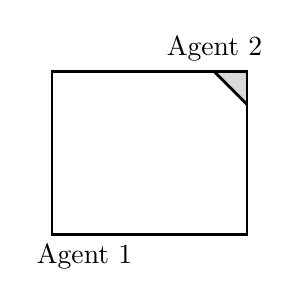
\begin{tikzpicture}[line width=1pt,scale=0.825]
\fill[black!15] (2.5,2.5) -- (3,2.5) -- (3,2);
\draw (2.5,2.5)--(3,2) (0.5,0) node[below]{Agent 1} (2.5,2.5) node[above]{Agent 2};
\draw (0,0) rectangle (3,2.5);
\end{tikzpicture}
\caption{Case with low aggregate risk ($\omega_1=1.2\omega_2$)\label{fig1a}}\vspace{-0.37cm}
\end{subfigure}
\hspace{1.0cm}
\begin{subfigure}[b]{0.6\textwidth}
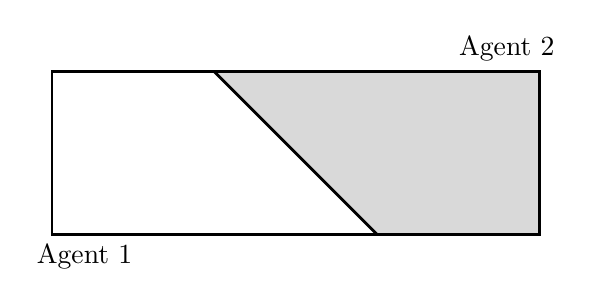
\begin{tikzpicture}[line width=1pt,scale=0.825]
\fill[black!15] (2.5,2.5) -- (5,0)  -- (7.5,0) -- (7.5,2.5);
\draw (2.5,2.5)--(5,0) (0.5,0) node[below]{Agent 1} (7,2.5) node[above]{Agent 2};
\draw (0,0) rectangle (7.5,2.5);
%
\end{tikzpicture}
\caption{Case with large aggregate risk ($\omega_1=3\omega_2$)\label{fig1b}}
\end{subfigure}
%\vspace{-0.5cm}
\end{center}\caption{Endowments distributions where equilibrium exists (gray region) in Example \ref{ex-1} \label{fig1}}
\end{figure}

%\vspace{-0.5cm}
As Figure \ref{fig1} shows, there is a clear difference between economies with substantial risk and economies with almost no risk. For example, in Figure \ref{fig1a}, the Edgeworth Box (EB) has an aggregate risk\footnote{Aggregate risk is defined as the ratio between the aggregate endowments $\omega_1$ and $\omega_2$.} of $20\%$, and, as a consequence, the possible endowment distributions for which equilibrium exists are restricted to endowment distributions with a very poor agent 2\footnote{Agent 2 might be more than 10 times poorer than agent 1.}. However when aggregate risk is large as in Figure \ref{fig1b}, the existence of equilibrium is less affected by large endowment distributions provided to the risk lover, increasing drastically the endowment allocations with equilibrium.
\begin{remark}
{Note that the risk lover does not have a null importance in the economy as \cite{Aumann2} suggested. What Condition \ref{aggriskex} requires is a large amount of aggregate risk to allow the trade between the agents as it was mentioned above. Figure \ref{figEB} illustrates how agents exchange the existing risk in the economy.}



\begin{figure}[h]
\begin{center}
%\vspace{-0.7cm}
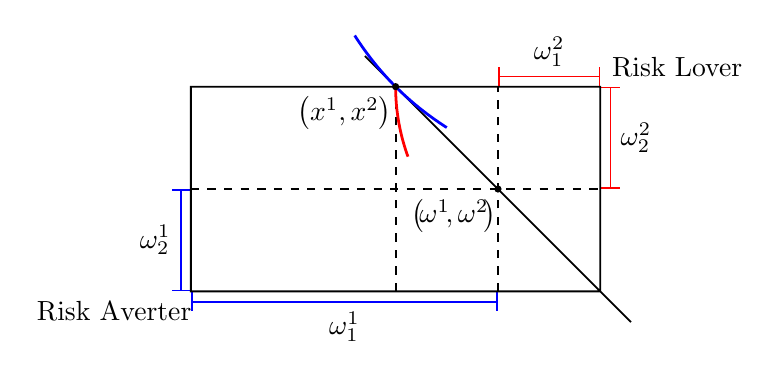
\begin{tikzpicture}[scale=1.3,line width=0.65pt]
\draw[|-|,blue] (0,-0.1) -- (3,-0.1);
\draw[|-|,blue] (-0.1,0) -- (-0.1,1);
\draw[|-|,red] (3,2.1) -- (4,2.1);
\draw[|-|,red] (4.1,1) -- (4.1,2);
\draw (0,0) rectangle (4,2) (1.7,2.3) -- (4.3,-0.3) (1.5,-0.1) node[below]{$\omega_1^1$} (-0.1,0.5) node[left]{$\omega_2^1$} (4.1,1.5) node[right]{$\omega^2_2$} (3.5,2.1) node[above]{$\omega^2_1$} (1.5,2) node[below]{$\left(x^1,x^2\right)$} (-0.75,0) node[below]{Risk Averter} (4.75,2) node[above]{Risk Lover} (2.57,1) node[below]{$\left(\!\omega^1\!,\omega^2\!\right)$};
\draw[dashed] (0,1) -- (4,1) (3,0) -- (3,2) (2,0) -- (2,2);
\draw[domain=1.6:2.5,blue, line width=1pt] plot(\x,4/\x);
\draw[domain=180:200,xshift=4cm,yshift=2cm,red,line width=1pt] plot({2*cos(\x)},{2*sin(\x)});
\fill (2,2) circle (1pt) (3,1) circle (1pt);
\end{tikzpicture}
\end{center}%\vspace{-0.7cm}
\caption{Edgeworth box\label{figEB}}
\end{figure}

\end{remark}


\end{example}

\subsection{Analysis for EU decision makers}


In this subsection, let us analyze an Edgeworth box with two  EU agents, $U^{i}\left(x\right)=\pi u^{i}\left(x_{1}\right)+\left(1-\pi\right)u^{i}\left(x_{2}\right),\ \forall i=1,2,$
where $\pi\!\in\!\left(0,1\right),u^{1}\in\!{C}^{1}\left(0,\infty\right)\cap{C}[0,\infty)$ is the utility index for the first agent, which is strictly increasing, concave in $[0,\infty)$ and $\lim_{x\rightarrow\infty}{u^1}'(x)=0$, and $u^{2}\in{C}[0,\infty)$ is the utility index for the second agent, which is an increasing and convex function satisfying $u^2(0)=0$.




\begin{prop}
\label{prop1}
Under our hypotheses, including Inada, there is $\underline{\omega}_1^1\geq0$ and $\underline{\omega}_2^1\geq0$ such that:
\begin{enumerate}
\item There is an AD-equilibrium if and only if (a) $\omega_1^1\geq\underline{\omega}_1^1$ and then $x_2^2=0$, or (b) $\omega_2^1\geq\underline{\omega}_2^1$ and then $x_1^2=0$. 

\item There is a unique normalized price $p=(p_1,1-p_1)\in\Delta_{++}^1$ for the AD-equilibrium, which is the solution of
\begin{equation}
\label{eq:-2}
\omega_1^1={{u^1}'}^{(-1)}\left(\left(\frac{p_1}{1-p_1}\right)\left(\frac{1-\pi}{\pi}\right){u^1}'\left(\omega_2\right)\right)+\frac{1-p_1}{p_1}\omega_2^2
%\omega_1^1={{u^1}'}^{(-1)}\left(\left(\left(\frac{p}{1-p}\right)\left(\frac{1-\pi}{\pi}\right){u^1}'\left(\omega_2\right)\right)\bigwedge{{u^1}'}(0)\right)+\frac{1-p}{p}\omega_2^2
\end{equation}
for (a), and the solution of
\begin{equation}
\label{eq:-21}
\omega_2^1={{u^1}'}^{(-1)}\left(\left(\frac{1-p_1}{p_1}\right)\left(\frac{\pi}{1-\pi}\right){u^1}'\left(\omega_1\right)\right)+\frac{p_1}{1-p_1}\omega_1^2
%\omega_2^1={{u^1}'}^{(-1)}\left(\left(\left(\frac{1-p}{p}\right)\left(\frac{\pi}{1-\pi}\right){u^1}'\left(\omega_1\right)\right)\bigwedge{{u^1}'}(0)\right)+\frac{p}{1-p}\omega_1^2
\end{equation}
for (b).
\end{enumerate}
\end{prop}
The proof of Proposition \ref{prop1} is in Appendix \ref{appA1}.


\begin{remark}
$\underline{\omega}_1^1$ and $\underline{\omega}_2^1$ are the values one would obtain for $\omega_1^1$ and $\omega_2^1$ respectively in \ref{eq:-2} and in \ref{eq:-21} taking $p$ as the solution of $\pi{u}^2\left(\nicefrac{p\omega^2}{p_1}\right)=(1-\pi)u^2\left(\nicefrac{p\omega^2}{(1-p_1)}\right)$.
Thus, $\underline{\omega}^1_1$ depends on all the other endowments of the economy. Similarly to $\underline{\omega}^1_2$.
\end{remark}

\begin{remark}
\label{remarknoInada}The previous result can be extended for a utility index that does not satisfy Inada. Then, for condition \ref{eq:-2}, we have 
\begin{equation}
\label{eq:-2n}
\omega_1^1={{u^1}'}^{(-1)}\left(\left(\left(\frac{p_1}{1-p_1}\right)\left(\frac{1-\pi}{\pi}\right){u^1}'\left(\omega_2\right)\right)\bigwedge{{u^1}'}(0)\right)+\frac{1-p_1}{p_1}\omega_2^2,
\end{equation}
 and, for condition \ref{eq:-21}, we have 
 \begin{equation}
 \label{eq:-21n}
 \omega_2^1={{u^1}'}^{(-1)}\left(\left(\left(\frac{1-p_1}{p_1}\right)\left(\frac{\pi}{1-\pi}\right){u^1}'\left(\omega_1\right)\right)\bigwedge{{u^1}'}(0)\right)+\frac{p_1}{1-p_1}\omega_1^2.
 \end{equation}
\end{remark}



The necessary and sufficient conditions of Proposition \ref{prop1} not only characterize the existence of equilibrium but also ensures its uniqueness. In addition, it is helpful to compute the equilibrium price and the optimal consumption for every equilibrium in this economy.

Proposition \ref{prop1} shows that to ensure the existence of equilibrium, a minimum level of endowment in one of the states of the risk averter is needed. Therefore, if we have economies in which the aggregate risk is relatively large and most of this wealth is in hands of the risk averter\footnote{In the sense of possession of endowments with large variations between the states.}, equilibrium would exist as a consequence of the exchange of risk with the risk lover. However, in some rare cases\footnote{It requires extremely large differences among agents and states.}, an equilibrium can exist in economies with no aggregate risk. 






\section{Equilibrium with non-convex agents: General case}
\label{section2}
\subsection{Model}
Let us define a model with $I+J$ agents where each agent $i$ is characterized by a utility function given by $U^i:\mathbb{R}^S_+\rightarrow\mathbb{R}$ and an Arrow-Debreu constraint given by $px\leq{p}\omega^i$, where $p\in\Delta^{S-1}_+$ is the price and $\omega^i\in \mathbb{R}^S_+$ is the initial endowment for the agent. In this economy, there are $S$ states of nature and one consumption good in each of them.

We will say that $\left(p,\left(x^i\right)_i\right)$ is an equilibrium (an Arrow-Debreu equilibrium), when $x^i$ is optimal for $U^i$ with the AD-constraint, and $\sum_i\omega^i=\sum_ix^i.$



From this point onwards, we will consider two different type of behaviors. The agents $i=1,\dots,I$ will be of Type $A$ and the agents $j=I+1,\dots,I+J$ will be of  Type $B$.

The agents of Type $A$ have the satisfy:
\begin{A} \label{A1}Utility function, $U^i$, strictly increasing, concave,\end{A}
\begin{A} \label{A2} For any $s$ and \label{eqA3}$\left\{ x^{n}\right\}_{n\in\mathbb{N}}\in\mathbb{R}_{+}^{S}$ such that $x_{s}^{n}\rightarrow\infty$ when $t\rightarrow\infty$, if $\nicefrac{x_{s'}^{n}}{x_{s}^{n}}\rightarrow0$ for $s'\neq{s}$ then\begin{equation}\lim_{n\rightarrow\infty}\left(\max_{T\in\partial{U\left(x^{n}\right)}}\frac{T\circ{e}_{s}}{T\circ{e}_{s'}}\right)=0\end{equation}
where $e_{s}$ is the $s$-canonical vector.
%For any $s$ and $\left\{x^n\right\}_{n\in\mathbb{N}}\in\mathbb{R}^S_{+}$, if $x^n_s\rightarrow\infty$ and $\left\{x^n_{s'}\right\}_{n\in\mathbb{N}}$ is bounded for $s'\neq{s}$ then\begin{equation}\lim_{n\rightarrow\infty}\left(\max_{T\in\partial{U^i\left(x^n\right)}}\frac{T\circ{e}_s}{T\circ{e}_{s'}}\right)=0\end{equation}where $e_s$ is the canonical vector with 1 in the component $s$ and 0 in any other case.
\end{A}

A\ref{A2} says about the marginal substitution rate between two states for large consumption levels, more precisely, when demand increases in state $s$ compared to state $s'$, the marginal demand in state $s$ converges to zero compared to the demand in state $s'$. In other words, It says that arbitrarily large consumption in some states, does not nullify the marginal utility of consuming any other good or state. Intuitively, there are no completely substitutable states or goods in the economy which is equivalent to say that there is some independence among the states or goods in the economy.

For the agents of Type $B$:
\begin{B} The utility function is strictly increasing and convex.\end{B}


The endowments are given by $\left(\omega_1^i,\dots,\omega_S^i\right)\gg0$. And let us denote $\omega_s:=\sum_{i=1}^{I+J}\omega_s^i,\ \forall{s=1,\dots,S}$.

Because type $B$ agents have convex utility functions, they have incentives to specialize their consumption as much as possible.

\begin{lemma}\label{lemmaL}
Given price $p$, all the $B$ agents have an optimal solution given by:\[x^{I+i}_s=\Bigg\{\begin{array}{lcl} 0 & & \textrm{for }{s}\neq s_0, \\ \frac{1}{p_{s^{\,}_{0_{\,}}}}\left[p\omega^{I+i}\right] & & \textrm{for some }s_0.\end{array}\]
Moreover, if the utility function $U^{I+i}$ is strictly convex, any optimal solution has the form of $x^{I+i}$ for some $s_0$.
\end{lemma}
The proof can be found in Appendix \ref{prooflemmaL}.

Note that if there is at least one agent of type $B$ that has a nonlinear utility function. We cannot apply the standard techniques of existence of equilibrium which include \cite{Shafer} and \cite{HeYannelis}.


As in Example \ref{ex-1}, we will show that the existence of aggregate risk helps the match of the hedging for type $A$ agents and the speculation of type $B$ agents. However, the former agents must have proportionally more wealth in one state to allow the specialization of the latter without violating market clearing.

\begin{thm}
\label{theo1}
{If the aggregate endowment of type $A$ agents is sufficiently large in a state $s$ compared with other states, there is an equilibrium for the economy.}

\end{thm}

{The proof can be found in Appendix \ref{prooftheo1}.

As it was mentioned above, Hypothesis A\ref{A2} implies some independence among states or goods which would help us to ensure that changes in the level of aggregate uncertainty will affect the marginal rates of substitution. %As it can be seen during the proof, this property becomes relevant to predict the type $B$'s behavior when there is a large amount of aggregate uncertainty in the economy.


Our result indicates that when there is enough wealth in one state for the $A$ agents, they are willing to transfer this new risk as much as they can to the $B$ agents, which allows the latter to improve their consumption.% Then, even in the presence of non-convex preferences, we will show that there is a balance among the agents given by the presence of this type of aggregate risk.


Note that if the \emph{B} agents cannot specialize very much, the aggregate risk needed in the economy to have an equilibrium is very low. Therefore, any regulation that reduces the specialization of the \emph{B} agents, it also reduces the amount of aggregate risk needed to ensure equilibrium.


\begin{remark}

Due to the mild hypotheses over the preferences, we can apply our result to \emph{Smooth Ambiguity} decision makers, see \cite{KMM}, \emph{Choquet Expected Utility} decision makers, see \cite{Schmeidler}, \emph{Rank-Dependent Expected Utility} decision makers, see \cite{Quiggin1,Quiggin2} \cite{Yaari} and \emph{Variational Preferences} \cite{MMR}.

\end{remark}

In the case of \emph{Expected Utility} decision makers, the previous result can also be extended to include the case in which the risk lovers specialize in different states (see Remark \ref{remks} in Appendix \ref{appA1}).

%\begin{remark}
%For the case with agents that are risk lovers in some states, $S^i_l$, and risk averters in other states, $S^i_a$, existence of equilibrium can be ensured for preferences such that for all $s\in\cap_{S^i_l\neq\emptyset}S^i_l$, the utility indexes in this state, $u^i_s(x)$, are linear for $x$ large enough. And similar to Theorem \ref{theo1}, some aggregate risk is necessary to ensure an equilibrium; in this case, the necessity of large endowment could be in more than one state. For example, consider an economy in which there is only two agents where $S^{I+1}_l,S^{I+2}_l\neq\emptyset$, and $S^{I+1}_l\cap{S}^{I+2}_l=\emptyset$, then it will be necessary to have two states with a large endowment in hand of the risk averters\footnote{Notice that this condition can be extended to more than two agents without the large symmetric hypothesis of Proposition \ref{propks}.}.
%\end{remark}
%



\section{Equilibrium in a static economy with Prospect Theory decision makers}
\label{sectionfs}


\subsection{Static Equilibrium with Prospect Theory}

In this section, we will define a similar model as before; nevertheless, we consider Prospect Theory decision makers instead of agents with convex utility functions (agents of type B). We will analyze the existence of equilibrium when there are also agents of type A\footnote{The type A agents will be from agent 1 to agent $I$.}.



Consider an AD economy similar to the one defined before with an objective probability $\pi$ and $\pi_s\geq\underline{\pi}>0$ is the probability of the state $s$\footnote{Notice that in our economy, agents can not buy lotteries as in the Ascombe-Aumann framework.}. Since this type of agents considers differently gains and losses based on their personal reference point it is necessary to make the analysis for gains and losses separately (gains for levels of wealth above the reference point and losses for levels of wealth below it).

{Therefore, if we interpret our economy as a two-dates economy in which, in $t=0$, contracts are made, and, in $t=1$, agents honor their promises; the reference point will the level of wealth that each agent will have before the contracts are honored in $t=1$, that is $\omega^{I+i}_s$, the initial endowment in state $s$.}
{If the agent does not have any shock in his/her wealth, the level of wealth will be constant among the states, $\omega^{I+i}_{s}=\omega^{I+i}_t$ for all $s,t$, however, if the agent has a shock caused by an external force, the reference points could not be necessarily the same in all states.}

%Since these agents change their attitude toward the reference point as we mentioned before, the Friedman-Savage utility index is useful in the analysis of the value function mentioned in the Prospect Theory literature. For the case of \cite{KT92}, we have:

Let us consider utility functions given by two Choquet Integrals, one for gains and one for losses. That is, $U^{I+i}(x)=U^{I+i,+}(x)+U^{I+i,-}(x)$ where $U^{I+i,+}(x)=(C)\int_{\{x_s\geq\omega^{I+i}_s\}}u^{I+i}(x)w^{I+i}(d\pi)$ is the utility functions only in the states above the reference point, $\omega^{I+i}_s$, and $U^{I+i,-}(x)=(C)\int_{\{-x_s<\omega^{I+i}_s\}}u^{I+i}(-x)w^{I+i}(d\pi)$ is the utility functions only in the states below the reference point. Each function is defined by a weighting function, $w^{I+i}$ and a value function, $u^{I+i}$\footnote{For simplicity of notation, we will use the same notation as in the case of the utility index as before.} that could change with each state $s$ since the reference point might change from one state to another one.

The weighting function, $w^{I+i}:[0,1]\rightarrow[0,1]$, is a strictly increasing continuous function such that there is a value $\hat{\pi}^{I+i}\in(0,1)$ such that $w^{I+i}$ is concave in $\left[0,\hat{\pi}^{I+i}\right)$, and $w^{I+i}$ is convex in $\left(\hat{\pi}^{I+i},1\right]$ with $w^{I+i}(0)=0$ and $w^{I+i}(1)=1$.



Since most of the Prospect Theory literature analyzes differently gains and losses in terms of the decision maker attitude toward risk, we will consider a value function, that changes for different levels of wealth. Therefore, the value function, ${u^{I+i}_s}:\mathbb{R}_+\rightarrow\mathbb{R}$, in each state $s$ is a differentiable, strictly increasing  function that is unbounded from below. Moreover, there are $0\leq{x}^i_{c,s}\leq\tilde{x}^i_s$ such that ${u^{I+i}_s}(x)$ is a concave differentiable function for $x\leq{x^{I+i}_{c,s}}$ or $x\geq\tilde{x}^{I+i}_s$, and ${u^{I+i}_s}(x)$ is a convex function for $x\in\left[x^{I+i}_{c,s},\tilde{x}^{I+i}_s\right]$. For decision makers as \cite{KT92}, we have:

\begin{TK} $x^{I+i}_{c,s}\leq0$ and $\tilde{x}^{I,i}_s=\omega^{I+i}_s\ \forall{s}$ where $x^{I+i}_{c,s}$ and $\tilde{x}^{I+i}_s$ are the inflection points for the state $s$.
\end{TK}

\begin{figure}[h]
\begin{center}
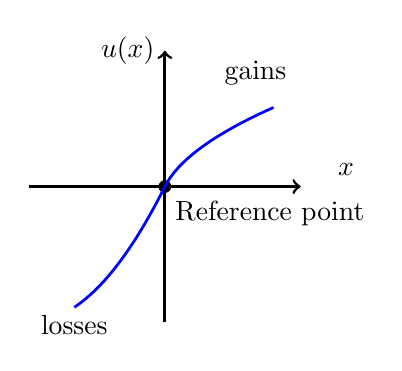
\begin{tikzpicture}[line width=1pt,scale=1.15]
\draw[->] (0,-1.5) -- (0,1.5);
\draw[->] (-1.5,0) -- (1.5,0);
%\draw (0,0) rectangle (4,4);
\draw (2,0) node[above]{$x$} (0,1.5) node[left]{$u(x)$};
\fill (0,0) circle (2pt);
%\fill (2,7/3) circle (2pt);
%\draw[dashed] (0,0) -- (2.25,2.25);
\draw[domain=-1:0,blue, line width=1pt] plot({\x},{2*(\x+2)*(\x+2)/3-2*(\x+2)/3+1-7/3});
\draw[domain=0:1.2,blue, line width=1pt] plot({\x},{sqrt((\x+2)-31/16)+25/12-7/3});
%\draw[dashed] (1,0) -- (1,1);
%\draw[dashed] (2,0) -- (2,7/3);
%\draw (1,0) node[below]{$x_c$};
\draw (0,-0.3) node[right]{Reference point};
\draw (1,1.5) node[below]{gains};
\draw (-1,-1.3) node[below]{losses};
\end{tikzpicture}
\end{center}
\caption{Form of the value function in the \cite{KT92} case.}
\end{figure}





Additionally, let us consider Prospect Theory decision makers with a value function given by \cite{JS} in which the decision makers will not be risk seeking for extremely low levels of wealth:
\begin{JS}
$x^{I+i}_{c,s}=\omega^{I+i}_s$ and $\tilde{x}^{I+i}_s>\omega^{I+i}_s\ \forall{s}$ where $x^{I+i}_{c,s}$ and $\tilde{x}^{I+i}_s$ are the inflection points for the state $s$.
\end{JS}

\begin{figure}[h]
\begin{center}
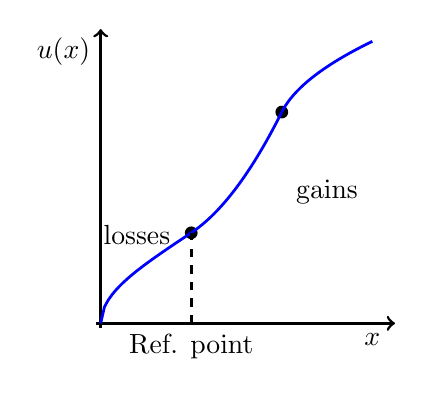
\begin{tikzpicture}[line width=1pt,scale=1.15]
\draw[->] (0,-0.05) -- (0,3.25);
\draw[->] (-0.05,0) -- (3.25,0);
%\draw (0,0) rectangle (4,4);
\draw (3,0) node[below]{$x$} (0,3) node[left]{$u(x)$};
\fill (1,1) circle (2pt);
\fill (2,7/3) circle (2pt);
%\draw[dashed] (0,0) -- (2.25,2.25);
\draw[domain=0:1,blue, line width=1pt] plot({\x},{(sqrt(\x)*4+\x*\x/2)/4.5});
\draw[domain=1:2,blue, line width=1pt] plot({\x},{2*\x*\x/3-2*\x/3+1});
\draw[domain=2:3,blue, line width=1pt] plot({\x},{sqrt(\x-31/16)+25/12});
\draw[dashed] (1,0) -- (1,1);
%\draw[dashed] (2,0) -- (2,7/3);
\draw (1,0) node[below]{Ref. point};
\draw (0.4,1.2) node[below]{losses};
\draw (2.5,1.7) node[below]{gains};
\end{tikzpicture}
\end{center}
\caption{Form of the value function in the \cite{JS} case.}
\end{figure}


Note that agents can not have arbitrarily large losses  in this framework since their consumption must be nonnegative in each state. One possible explanation to this is that in a more complex framework than the one considered by the classical Prospect Theory, agents can not have arbitrarily large losses in an environment without default since they are exogenously forced to avoid negative consumption.


%Now, let us assume an additional hypotheses of agents of type A:
%
%\begin{A}
%\label{A3}
%For any $s$ and \label{eqA3}$\left\{ x^{n}\right\}_{n\in\mathbb{N}}\in\mathbb{R}_{+}^{S}$, if $x_{s}^{n}\rightarrow\infty$ and $\nicefrac{x_{s'}^{n}}{x_{s}^{n}}\rightarrow0$ for $s'\neq{s}$ then\begin{equation}\lim_{n\rightarrow\infty}\left(\max_{T\in\partial{U\left(x^{n}\right)}}\frac{T\circ{e}_{s}}{T\circ{e}_{s'}}\right)=0\end{equation}
%where $e_{s}$ is the canonical vector with 1 in the component s and 0 in any other case.
%\end{A}


The following result ensures the existence of equilibrium for economies with agents with preferences as the one described above. %For simplicity, let us assume that $\omega^{I+i}_s=\omega^{I+i}_{s'}=\omega^{I+i}$ for all $s,s'=1,\dots,S$ for each $i=1,\dots,J$, that is, the endowment allocation will not change among the states  for each Prospect Theory decision maker.


\begin{prop}
\label{exisFS}

In a economy in which $I$ agents satisfy \textbf{A\ref{A1}}-\textbf{A\ref{A3}} and $J$ agents satisfy \textbf{TK} or \textbf{JS}, if the aggregate endowment of the A agents satisfies that $\sum_{i=1}^{I}\omega_{s_{1}}^{i}\gg\sum_{i=1}^{I}\omega_{s_{2}}^{i}\gg\dots\gg\sum_{i=1}^{I}\omega_{s_{S}}^{i}\geq\max_s\left\{\sum_{j=1}^{J}\omega_{s}^{I+j}\right\}$, there is an equilibrium for the economy with $p\in\Delta_{++}^{S-1}$. 

%{If the aggregate endowment of type $A$ agents is sufficiently large in $0<S_1<S$ states compared with other states, there is an equilibrium for the economy.}
%Given a state $1\leq{s}\leq{S}$, there is $K>0$ such that $\sum_{i\leq{I}}\omega_s^i\geq{K}$, and then there is an equilibrium for the economy and the equilibrium price satisfies that $p\in\Delta_{++}^{S-1}.$
\end{prop}



%\begin{remark}
%{To analyze a more general case than the one mentioned above, for example, with nonlinear distortions, the result will be still valid under some additional conditions, for example, conditions that ensure a non constant consumption among the agents and, as a consequence, the utility function can be written in functional form in a neighborhood of the optimal solution. Under these conditions, it can be extended for cases where there are two different distortions which are concave for small probabilities and convex for large probabilities as in \cite{KT92}, \cite{ABW}, \cite{Wakker} or else \cite{JS}.}
%\end{remark}

In economies with infinitely many states, the conditions mentioned above are not sufficient to ensure equilibrium since the distortions of low-probability events could cause a type of arbitrage for standard EU agents or risk-neutral firms in a complete markets framework with an infinite number of states of nature,  see \cite{AG}. However, an infinite-state model with incomplete markets could be compatible with equilibrium with decision makers given by Prospect Theory since this economy could lead to an economy with several AD constraints.





\subsection{Existence with Friedman-Savage decision makers}



Each Friedman-Savage (FS) Decision Maker $i=I+1,\dots,I+J$ has a subjective probability $\pi^i\in\Delta^{S-1}_{++}$ and a utility index ${u^i}$  that is differentiable, strictly increasing, concave for $x<{x^i_{c}}$ and $x\geq\tilde{x}^i$, and, convex for $x\in\left[x^i_{c},\tilde{x}^i\right]$. Note that in this case, there is no relationship between the endowment allocation and the inflection points of the utility index.

%{This type of agent has a very particular behavior due to the two inflection points, before the first inflection point wherein each FS Decision Maker behaves as risk averter, avoiding extreme consumptions; although, when this agent is wealthier, he will behave as a certain type of risk lover, avoiding consumption without risk, however, if the agent becomes even more wealthier, his attitude toward risk changes again becoming  a risk averter. Intuitively, this implies that he is worried about the extremely low consumptions  even having incentives to specialize at some levels of wealth, and, at the same time, he does not have strong incentives to have a large specialization when their wealth is considerably large; this behavior is supported by several empirical works in which bettors changes their attitude toward risk becoming risk averters for gains  and risk lovers for losses based on a reference point, their wealth as in \cite{JS}.}
%
%%{The agents described above are willing to specify in some states but are also concerned about low consumption in all the states; at the same time, this agents that are willing to absorb risk at some middle level of income but they are not willing to do so when they are in high level of it. }
%
%{This behavior cannot be explained with the previous type of preferences because each B agent is willing to specialize in one state in absence of any type of constraint and its attitude does not depend on the level of wealth.}

\begin{cor}
\label{corollary}
{For preferences described above under the conditions of Proposition \ref{exisFS}, there is an equilibrium for the economy.}
\end{cor}



%\begin{remark}
%{For each Friedman-Savage decision maker, if Inada condition holds,
%%$\lim_{x\searrow0}{u^i}'(x)=\infty$
% in equilibrium, each DM would have a positive consumption in each state. However, if Inada condition is not satisfied, they might have null consumption in some states even when they have incentives to avoid them.}
%\end{remark}

\begin{remark}
If the endowment for all FSDM is quite small, or quite large, compared to $x^i_c$ and $\tilde{x}^i$ respectively, no aggregate endowment uncertainty is needed since all of them will consume in the first concave part, or in the second convex part, of the utility index.
\end{remark}

The lack of aggregate risk could prevent the existence of equilibrium if the Friedman-Savage decision makers are not extremely ``poor'' or extremely ``rich''. Example \ref{exFSne} in Appendix \ref{appex}.



%\begin{remark}
%\label{remarkfsext}
%With respect to the general utility index of Friedman and Savage, it is possible to show the existence of equilibrium for agents that are quite poor or considerably rich such that their consumption is always in the concave part of the utility index. \textbf{However, it is possible to extend the Lemma \ref{lemma3} in page \pageref{lemma3} to  all types of FS utility indexes implying that the consumption in the convex part is at most in one state. For agents with consumption in the convex part, the proof of Proposition \ref{exisFS} can not be extended however, numerically can be observed that the result remains true.}
%\end{remark}




%\subsubsection{A numerical analysis of prices with Friedman-Savage preferences}
%Because increments on the Friedman-Savage Wealth produce changes in their decisions against risk, our goal will be to establish a relationship between the risk absorbed by them and their wealth and -- as a consequence -- a relationship between prices and wealth of the FS decision makers.% The following example illustrates these relationships.
%
%\begin{example}
%Consider an economy with two states of nature with the probability $\pi=0.5$ that the first state occurs, two EU agents, where $u^1(x)=\ln(x)$ and $u^2(x)=\left\{\begin{array}{ll}\ln(x)+(1/2)x^2 & \textnormal{if }x\leq3/2 \\ 13/6(x-3/2)+9/8+\log(3/2) & \textnormal{if }x>3/2,\end{array}\right.$ and endowments given by $\omega^1=(5-2.5a,2-a)$ and $\omega^2=(2.5a,a)$ where $a\in[0,1]$.
%\begin{center}
%\begin{figure}[ht]
%\includegraphics[width=0.48\linewidth]{propconsfs1.pdf}
%\includegraphics[width=0.5\linewidth]{volatilityfs1.pdf}
%\vspace{-0.3cm}
%\caption{Changes in consumption and Absolute Variation of Prices against Wealth\label{grapfs}}
%\end{figure}
%\end{center}
%\vspace{-0.5cm}
%From the analysis of the Figure \ref{grapfs}, incremental increases of wealth of the FS agent lead to reductions of the absolute variation of prices. This is a consequence of the increasing desire of this decision maker to specialize when there are incremental increases of his wealth. Under a low wealth condition, the economy will be convex because both agents would have convex preferences under the feasible space. However under a substantial wealth condition, the FS decision maker will have enough incentives to specialize the consumption in one state.
%
%Because we are using allocations in the sense of Proposition \ref{exisFS}, there is some type of aggregate risk in the economy. Therefore, as the Friedman-Savage decision maker is becoming richer, she will have incentives to specialize her consumption and absorb larger quantities of risk, which reduces the volatility of the economy with a pro$-$cyclical asset.
%
%
%
%\end{example}
%
%


\section{Conclusions}
\label{sectconc}
Given the importance of risk loving and ambiguity loving in financial markets, the exchange of aggregate risk between risk/ambiguity lovers and the risk/ambiguity averters is an important problem to be studied since it has not been analyzed in the General Equilibrium Theory.

We gave conditions in terms of enough aggregate risk for a large class decision makers encompassing \emph{SA} (see \cite{KMM}), \emph{CEU} (see \cite{Schmeidler}), \emph{VPs} (see \cite{MMR}) and Prospect Theory\footnote{More precisely, in the sense of \cite{JS} and \cite{KT92}.} under which we were able to prove the existence of equilibria\footnote{For existence of Pareto Optima see \cite{ABCN}.}. These conditions suggest a minimum level of aggregate risk is needed to enable the trade between both types of agents allowing the matching between the desire of hedging of risk/ambiguity averters and the desire of speculation of risk/ambiguity lovers.

The analysis mentioned above can be useful to analyze theoretically and numerically the influence of risk/ambiguity loving or Prospect Theory decision makers in economies with financial markets and how volatility and welfare can be affected by these agents.


\appendix

\section{Appendix}
%\subsection{Proofs of existence of equilibrium}
%\label{appA}
\subsection{Proofs of Section \ref{section2}}\label{appA1}





\label{prooflemmaL} \begin{proof}{[}Proof of Lemma \ref{lemmaL}{]}
Since all $B$ agents have a convex utility function, for any $\alpha\in[0,1]$,
$U^{i}(\alpha{x}_{1}+(1-\alpha)x_{2})\leq\alpha{U}^{i}(x_{1})+(1-\alpha)U^{i}(x_{2})\leq\max_{t}\{U^{i}(x_{t})\}$,
which implies that there is an optimal consumption on the boundary
of the budget set,$\left\{ \left(0,\dots,\frac{1}{p_{s}}\left[p\omega^{i}\right],\dots,0\right)\right\} _{s=1}^{S}$.
\end{proof}

\begin{proof}{[}Proof of Proposition \ref{prop1}{]} Let us prove
that there is an equilibrium for the economy. For any $p_{1}\in(0,1)$,
since the agent 2 has a strictly convex and strictly increasing utility
index, the optimal solution must be on the frontier of the budget
set therefore the possible optimal solutions are $\left(\frac{p\omega^{2}}{p_{1}},0\right)$
and $\left(0,\frac{p\omega^{2}}{1-p_{1}}\right)$, see lemma \ref{lemmaL}.

From now on, we will analyze the case in which the agent 2 specializes
in the first state. Consider $\overline{p}_{1}\in\left(0,1\right)$
and $\overline{p}=(\overline{p}_{1},1-\overline{p}_{1})$\footnote{The uniqueness of $\overline{p}_{1}$ is a consequence of $u^{2}$
being strictly increasing, $u^{2}(0)=0$, $u^{2}(x)\rightarrow\infty$
when $x\rightarrow\infty$, and that the left part of \ref{eq:-3}
is decreasing and the right part is increasing on $\overline{p}_{1}$.} as the solution of 
\begin{equation}
\pi u{}^{2}\left(\frac{\overline{p}\omega^{2}}{\overline{p}_{1}}\right)=\left(1-\pi\right)u^{2}\left(\frac{\overline{p}\omega^{2}}{1-\overline{p}_{1}}\right),\label{eq:-3}
\end{equation}
 $\underline{\omega}_{1}^{1}>0$ as the solution of Equation \ref{eq:-2}
with $p_{1}=\overline{p}_{1}$ and $\omega:(0,1)\rightarrow(0,\infty)$
as $\omega(p)={{u^{1}}'}^{\left(-1\right)}\!\!\left(\!\left(\frac{p}{1-p}\right)\!\!\left(\frac{1-\pi}{\pi}\right)\!{u^{1}}'\left(\omega_{2}\right)\right)+\frac{1-p}{p}\omega_{2}^{2}$ \footnote{$\underline{\omega}_{1}^{1}$ and $\omega(\cdot)$ are well defined
since $u^{1}$ being strictly concave, ${u^{1}}'(0)=\infty$ and ${u^{1}}'(\infty)=0$.}, which is strictly decreasing on $p$.

Now let us prove that for each $\omega_{1}^{1}\geq\underline{\omega}_{1}^{1}$,
there is an equilibrium when the price $(p_{1},1-p_{1})$ satisfies
$p_{1}=\omega^{-1}(\omega_{1}^{1})$.

If $\omega_{1}^{1}\geq\underline{\omega}_{1}^{1}$, then $p_{1}\leq\overline{p}_{1}$
so $\pi u{}^{2}\left(\frac{p\omega^{2}}{p_{1}}\right)\geq\left(1-\pi\right)u^{2}\left(\frac{p\omega^{2}}{1-p_{1}}\right).$

This implies that the optimal consumption of the agent 2 is $\left(\!\frac{p\omega^{2}}{p_{1}},\!0\!\right)$.

Now, the FOC for the agent 1 implies that $\pi{u^{1}}'\left(x_{1}^{1}\right)=p_{1}\mu,$
$\left(1-\pi\right){u^{1}}'\left(x_{2}^{1}\right)=\left(1-p_{1}\right)\mu$
and 
\begin{equation}
\ \ \ \ \ \ \ \ p_{1}x_{1}^{1}+\left(1-p_{1}\right)x_{2}^{1}=p_{1}\omega_{1}^{1}+\left(1-p_{1}\right)\omega_{2}^{1},\label{eq:-4}
\end{equation}

for $\mu>0$. Therefore, $\mu=\frac{1-\pi}{1-p}{u^{1}}'(\omega_{2})$
and 
\[
\left(x_{1}^{1},x_{2}^{1}\right)=\left({{u^{1}}'}^{\left(-1\right)}\left(\left(\frac{p}{1-p}\right)\left(\frac{1-\pi}{\pi}\right){u^{1}}'\left(\omega_{2}\right)\right),\omega_{2}\right)
\]
 is the optimal solution for agent 1. 

Since we have $x_{2}^{1}+x_{2}^{2}=\omega_{2}$ and $x_{1}^{1}+x_{1}^{2}={{u^{1}}'}^{\left(-1\right)}\left(\left(\frac{p}{1-p}\right)\left(\frac{1-\pi}{\pi}\right){u^{1}}'\left(\omega_{2}\right)\right)+\omega_{1}^{2}+\frac{1-p}{p}\omega_{2}^{2}=\omega_{1}^{1}+\omega_{1}^{2}$,
this concludes the proof of existence of equilibrium when $x_{1}^{2}\neq0$,
that is, the risk lover specializes in state 1. The proof is analogous
when $x_{2}^{2}\neq0$.

Now, let us prove the converse, suppose that there is an equilibrium
$\left(\hat{p},\ \hat{x}\right)$ with $\hat{x}_{1}^{2}\neq0$ for
the economy defined by endowments $\left(\omega^{1},\omega^{2}\right)$,
then $\hat{x}_{2}^{1}=\omega_{2}$. Since the risk lover is specializing
in state 1, $\hat{p}$ satisfies 
\[
\pi{u}^{2}\left(\frac{\hat{p}\omega^{2}}{\hat{p}_{1}}\right)-(1-\pi){u}^{2}\left(\frac{\hat{p}\omega^{2}}{1-\hat{p}_{1}}\right)\geq0.
\]

Now, let us define a function $f:(0,1)\rightarrow\mathbb{R}$ as $f(p):=\pi{u}^{2}\left(\frac{\left({p},1-{p}\right)\omega^{2}}{{p}}\right)-(1-\pi){u}^{2}\left(\frac{\left({p},1-{p}\right)\omega^{2}}{1-{p}}\right)$,
note that $f$ is strictly decreasing and that $\overline{p}_{1}$
is the greatest $p\in(0,1)$ such that $f(\overline{p})=0$, therefore
$\hat{p}_{1}\leq\overline{p}_{1}$. And due to the FOC of agent $1$
and market clearing, $x_{2}^{1}=\omega_{2}$, $x_{1}^{1}={{u^{1}}'}^{\left(-1\right)}\left(\left(\frac{\hat{p}}{1-\hat{p}}\right)\left(\frac{1-\pi}{\pi}\right){u^{1}}'\left(\omega_{2}\right)\right)$
and $x_{1}^{1}+x_{1}^{2}={{u^{1}}'}^{\left(-1\right)}\left(\left(\frac{\hat{p}}{1-\hat{p}}\right)\left(\frac{1-\pi}{\pi}\right){u^{1}}'\left(\omega_{2}\right)\right)+\omega_{1}^{2}+\frac{1-\hat{p}}{\hat{p}}\omega_{2}^{2}=\omega_{1}^{1}+\omega_{1}^{2}$
which is equivalent to 
\[
\omega_{1}^{1}={{u^{1}}'}^{\left(-1\right)}\left(\left(\frac{\hat{p}}{1-\hat{p}}\right)\left(\frac{1-\pi}{\pi}\right){u^{1}}'\left(\omega_{2}\right)\right)+\frac{1-\hat{p}}{\hat{p}}\omega_{2}^{2}
\]
which clearly implies that $\omega_{1}^{1}\geq\underline{\omega}_{1}^{1}$.
Which concludes the proof. 

{[}Proof of Remark \ref{remarknoInada}{]} Due to the FOC, to guarantee
that agent $1$ has a positive consumption in each state it is enough
to show that 
\begin{equation}
\left(\frac{1-p_{1}}{p_{1}}\right)\left(\frac{\pi}{1-\pi}\right){u^{1}}'\left(\frac{p_{1}\omega_{1}^{1}+\left(1-p_{1}\right)\omega_{2}^{1}}{p_{1}}\right)<{u^{1}}'\left(0\right)\label{eq:-7}
\end{equation}
for any $p_{1}\leq\overline{p}_{1}$ where $\omega_{1}^{1}$ satisfies
the equation \ref{eq:-2n}. And since ${u^{1}}'$ is strictly decreasing
and $\omega_{2}^{1}>0$, we have that 
\[
\left(\frac{1-p_{1}}{p_{1}}\right)\left(\frac{\pi}{1-\pi}\right){u^{1}}'\left(\frac{p_{1}\omega_{1}^{1}+\left(1-p_{1}\right)\omega_{2}^{1}}{p_{1}}\right)<\frac{(1-p_{1})\pi}{p_{1}(1-\pi)}{u^{1}}'\left(\omega_{1}^{1}\right)
\]
and then, using \ref{eq:-2n} and the properties of $u^{1}$, we have:
\[
\frac{(1-p_{1})\pi}{p_{1}(1-\pi)}{u^{1}}'\left(\omega_{1}^{1}\right)<\frac{(1-p_{1})\pi}{p_{1}(1-\pi)}\left(\left(\frac{p_{1}(1-\pi)}{(1-p_{1})\pi}{u^{1}}'\left(\omega_{2}\right)\right)\wedge{u^{1}}'\left(0\right)\right)<{u^{1}}'(0).
\]
Finally, we can apply the proof of Proposition \ref{prop1} to finish
the proof.

\end{proof}


\begin{remark}
\label{remks}
Given $\left\{\omega_s^i\right\}_{s,i}$ if there are $R$ states, $1\leq{s_1},\dots,s_R\leq{S}$ and $0<k<K$, with $K$ sufficiently large such that:
\begin{enumerate}
\item (Symmetry)\label{cond1} The probability, $\pi_{s_r}$, is the same for all $r$ and $J=R\tilde{J}$ with $\tilde{J}\in\mathbb{N}$ and $\omega^{I+j_1}=\omega^{I+j_2}$ for $j_1=\tilde{j}R+l_1$ and $j_2=\tilde{j}R+l_2$ where $1\leq{l}_1,l_2\leq{R}$ and $0\leq\tilde{j}<R$,
\item (Boundedness) $\sum_{i\leq{I}}\omega_{s_r}^i=\sum_{i\leq{I}}\omega^i_{s_{r'}}\geq{K}$ and $\sum_{i>I}\omega_{s_r}^i\leq{k}$ for all $r,r'=1,\dots,R$, and $\sum_{i}\omega_{s'}^i\leq{k}$ for $s'\neq{s}_r$ for all ${r}=1,\dots,R$.
\end{enumerate}
Then, there is an equilibrium for the economy with $p\in\Delta_{++}^{S-1}.$
\end{remark}


\begin{proof}
We define a fictitious economy in which each $\tilde{j}R+1,\dots,\left(\tilde{j}+1\right)R$ will specialize in $s_1,\dots,s_R$ respectively. And, using \ref{cond1}, we ensure that in fictitious economy, the prices must satisfy $p_{s_1}=\dots=p_{s_R}$, which concludes the proof.
\end{proof}

\subsection{Proof of Theorem \ref{theo1}}

\label{prooftheo1} \begin{proof} Without loss of generality we will
analyze the case in which $\sum_{i\leq{I}}\omega_{1}^{i}$,
the aggregate endowment of the type $A$ agents is large in the first
state compared to aggregate endowment in other states and the aggregate
endowment of the type $B$ agents in the first state. Therefore, Theorem \ref{theo1} can be rewritten as follows, \emph{there is $\overline{K}\geq0$ such that for every endowment allocation that satisfies $\frac{\sum_{i\leq{I}}\omega_{1}^{i}}{\max\left\{\sum_{j\leq{J}}\omega_{1}^{I+j},\max_{s=2,\dots,S}\overline{\omega}_s\right\}}\geq \overline{K}$, the economy has an equilibrium.} Therefore, if we define \begin{equation}\label{defK}K=\frac{\sum_{i\leq{I}}\omega_{1}^{i}}{\max\left\{\sum_{j\leq{J}}\omega_{1}^{I+j},\max_{s=2,\dots,S}\overline{\omega}_s\right\}},\end{equation} to prove Theorem \ref{theo1} it is enough to ensure that there will be an equilibrium for any economy that satisfies that $K$ is large enough.
%To do so, let
%be $\left\{ \left(\omega_{1}^{i},\dots,\omega_{S}^{i}\right)\right\} _{i=1}^{I+J}\gg0$
%the initial endowments satisfying that $\omega_{1}^{K,i}:=\underline{\omega}_{1}^{i}+\beta_{i}{K}$
%where $\beta\in\Delta_{+}^{I-1}$, $\left\{ \underline{\omega}_{1}^{i}\right\} _{i\leq{I}}>0$.
%Our goal is to show that for every $\left\{ \left(\omega_{2}^{i},\dots,\omega_{S}^{i}\right)\right\} _{i=1}^{I+J}\gg0$,
%$\left\{ \omega_{1}^{i}\right\} _{i>{I}}$, $\beta\in\Delta_{+}^{I-1}$
%and $\left\{ \underline{\omega}_{1}^{i}\right\} _{i\leq{I}}$ there
%exists $\underline{K}\geq0$ such that if $K\geq\underline{K}$, there
%is an equilibrium for the economy. For notation, let us denote $\omega_{s}^{K,i}=\omega_{s}^{i}$
%for $s=2,\dots,S$ and $i=1,\dots,I+J$, and $\omega_{1}^{K,i}=\omega_{1}^{i}$for
%all $i=1,\dots,I$.

The idea is to define a fictitious convex economy that satisfies the
standard conditions for existence of equilibrium and then, for $K$
large enough, the equilibrium of the fictitious economy is in fact
an equilibrium for the initial non-convex economy. To do so, we will
use some special properties that the equilibrium price have when $K$
is large enough.

Let us define the fictitious economy with the same number of agents,
$I+J$, and the same endowments $\left\{ \left(\omega_{1}^{i},\dots,\omega_{S}^{i}\right)\right\} _{i=1}^{I+J}$
with utility functions $\left\{ V^{i}\right\} _{i}$.

Each agent $i=1,\dots,I$ is defined by the same utility function,
that is $V^{i}=U^{i}$, and the same budget constraint as in the initial
economy. However, for an agent $i=I+1,\dots,I+J$, the utility function
is $V^{i}(x):=x_{1}$ and the same budget constraint. As a consequence, there is an equilibrium
$\left(\left(x^{i}\right)_{i=1}^{I+J},p\right)$ for the fictitious
economy. 

Now, in order to prove that the equilibrium for the fictitious economy
is, in fact, an equilibrium for the initial economy, it is necessary
to prove that the allocation $x^{i}$ is optimal for the consumers
in the initial economy. Note that for an agent $i=1,\dots,I$ in
the original economy, the allocation $x^{i}$ is also optimal.

Our goal is to ensure that there is $\underline{K}\geq0$ such that
if $K\geq\underline{K}$, the agent $i=I+1,\dots,I+J$ maximizes his
consumption at $x^{i}$ for every $i$. The idea of this part is
to ensure that for $K$ large enough, all agents will have enough
incentives to buy more in state one than in the other states in such
a way that all the agents of type $B$ will consume in the first state
or good. These incentives are perceived by the agents as a lower price
in state 1 compared to the other states. 

\begin{lemma} \label{lemma1} Under the same assumptions, for every sequence of fictitious economies with endowment allocation $\left\{\omega^{i,n}\right\}_{n\in\mathbb{N}}$ such that $\{K^n\}_{n\in\mathbb{N}}$ defined by Equation \ref{defK} satisfies that $\lim_{n\rightarrow\infty}K^n=\infty$ $\nicefrac{p_{1}^{n}}{p_s^n}\rightarrow0$ for every $s\neq1$ when $n\rightarrow\infty$. \end{lemma}

\begin{proof}Since $p^{n}\in\Delta_{+}^{S-1}$, without loss of generality, we can assume that $p^{n}\rightarrow\hat{p}\in\Delta_{+}^{S-1}$. Now, let us separate
the proof in two parts: 
\begin{enumerate}
\item Let us show that $\hat{p}_{1}=0$. So, assume that $\hat{p}_{1}>0$.

Since $K^n\rightarrow\infty$, there exists at least one agent $\left(\overline{i}\leq{I}\right)$ and a subsequence $\left\{n_k\right\}_{k\in\mathbb{N}}$
such that $p^{n_k}\omega^{n_k,\overline{i}}$ is unbounded, and the
agent's consumption in the first state is also unbounded (which implies
that for $k$ large enough, $x_{1}^{n_k,\overline{i}}>0$) implying that the
FOC in state $1$ is satisfied with equality. Therefore,
for $k$ large enough and $\varepsilon\in(0,\hat{p}_{1})$, there is $T^{n_k,\overline{i}}\in\partial{U}^{\overline{i}}\left(x^{n_k,\overline{i}}\right)$\footnote{By $\partial U$ we mean the supperdifferential of the function $U$.}
such that $\frac{T^{n_k,\overline{i}}\circ{e_{1}}}{T^{n_k,\overline{i}}\circ{e_{s}}}\geq\frac{p_{1}^{n_k}}{p_{s}^{n_k}}\geq{\hat{p}_{1}-\varepsilon}>0$, which implies that $x_{s}^{n_k,\overline{i}}\rightarrow\infty$ as a consequence of A\ref{A2}, contradicting market clearing.



%The intuition for this part of the proof is that if the price of the
%state $1$ is not going to $0$, at least one $A$ agent will consume
%quantities arbitrarily large in a state different from the first one
%which is a contradiction due to the scarcity of the good in state
%$s\neq1$.
\item Let us show now that $\nicefrac{p_{1}^{n}}{p_s^n}\rightarrow0$ when $n\rightarrow\infty$ for every $s\neq1$. So, let us
assume that there exists at least one $s=2,\dots,S$ and $\underline{\alpha},\overline{\alpha}\in(0,\infty)$ such that $\underline{\alpha}\leq\nicefrac{p_{1}^{n}}{p_s^n}\leq\overline{\alpha}$.

Due to market clearing, there exists an agent $i_{n}\leq{I}$
such that $x_{s}^{n,i_{n}}\geq\nicefrac{\overline{\omega}_{s}^{n_k}}{(I+J)}>0$ implying that the FOC is satisfied with equality
for the agent $i_{n}$ in states 1 and $s$. As a consequence, there
is $T^{n,i_{n}}\in\partial{U}^{{i}_n}\left(x^{n,i_{n}}\right)$ such
that $\underline{\alpha}\leq\frac{T^{{n,i_{n}}}\circ{e_{1}}}{T^{{n,i_{n}}}\circ{e_{s}}}=\frac{p_{1}^{n}}{p_{s}^{n}}\leq\overline{\alpha}$, which implies that there are $\underline{\beta},\overline{\beta}>0$ such that $\underline{\beta}\leq\frac{x_{1}^{n,i_n}}{x_{s}^{n,i_n}}\leq\overline{\beta}$\footnote{Note that $p^{n_k}_1\rightarrow0$ when $k$ goes to infinity implies that $x^{n_k,i}\rightarrow\infty$ for all $i=1,\dots,I$.} contradicting market clearing.

%The proof of the second case has a different intuition, it says that
%if there is another state price going to $0$, then at least one agent
%is consuming more in this state than in the others with positive limit
%price when $n$ goes to infinity which is incompatible with the scarcity
%of the good in state $s\neq1$.
\end{enumerate}
\end{proof}

Now, let us prove that $\left(x^{i}\right)_{i=I+1}^{I+J}$ is
optimal for the $B$ type of agents for $K$ large enough. Since each
agent $i=I+j\geq{I+1}$ in the initial economy has a strictly convex
utility function, the optimal solutions are contained in $\Bigg\{\left(\frac{p\omega^{I+j}}{p_{1}},0,\dots,0\right)$,
$\dots,\left(0,\dots,0,\frac{p\omega^{I+j}}{p_{S}}\right)\Bigg\}$.
If we use Lemma \ref{lemma1}, we have that for $K$ large enough, $\frac{p_{1}}{p_{s}}\sim0$ for all $s\neq1$, then, $\nicefrac{\frac{p\omega^{I+j}}{p_{s}}}{\frac{p\omega^{I+j}}{p_{1}}}\sim0$, and, since $U^{I+j}$
is a strictly convex and strictly increasing function for each $j\leq{J}$, $\lim_{n\rightarrow\infty}\nicefrac{U^{I+j}(a_n e_s)}{U^{I+j}(b_n e_{s'})}=\infty$\footnote{$e_1=(1,0,\dots,0)$, $e_2=(0,1,0,\dots,0)$, $\dots$, and $e_S=(0,\dots,0,S)$} for every $s,s'=1,\dots,S$, $i\leq J$ and all nonnegative sequences $\left\{a_n\right\}_n$, $\left\{b_n\right\}_n$ such that $\lim_na_n=\lim_n\frac{a_n}{b_n}=\infty$, which implies that $U^{I+j}\left(\frac{p\omega^{I+j}}{p_{1}},0,\dots,0\right)\geq{U}^{I+j}\left(0,\dots,0,\frac{p\omega^{I+j}}{p_{s}},0,\dots,0\right)$,
for all $s\geq2,\ j=1,\dots,J$ for $K$ is large enough then, his optimal
solution coincides with the optimal solution of the agent $I+j$ in
the fictitious economy. Therefore, $\left(\left(x^{i}\right)_{i=1}^{I+J},p\right)$
is an equilibrium for the initial economy for $K$ large enough concluding the proof.\end{proof}

\subsection{Proof of Proposition \ref{exisFS}}

\label{appC}

\begin{proof}
Let us define the parameter $K$ as
\begin{equation}
\label{defKp}
K=\min_{s=1\dots,S-2}\left\{\frac{\sum_{i\leq I}\omega^i_s}{\sum_{i\leq I}\omega^i_{s+1}}\right\}.
\end{equation}
Note that if $K$ is large enough, we know that there is a large aggregate risk in the economy that it is in hands of the agents of type $A$.

Our goal will be to prove that for an economy with $K$ large enough, there is an equilibrium.

Our approach is similar to the proof of Theorem \ref{theo1} however,
there are some parts that must to be modified. The first thing to
be adapted concerns the agents in the fictitious economy that would represent
the Prospect Theory type of agents in the initial economy.

Consider a fictitious economy with $I+J$ agents with the same budget
constraint for all agents, for each agent $i=1,\dots,I$, the same utility function $\tilde{U}^i$ is defined as $\tilde{U}^{i}(x)=U^{i}(x)$,
and, for each agent $i=I+1,\dots,I+J$, $\tilde{U}^{i}(x):=\sum_{s}\gamma_{s}^{i}\tilde{u}_{s}^{i}(x_{s})$
with $\gamma_{1}^{i}=w^{i}\left(\pi_{1}\right)$, $\gamma_{s}^{i}=w^{i}\left(\sum_{k=1}^{s}\pi_{k}\right)-w^{i}\left(\sum_{k=1}^{s-1}\pi_{k}\right)$
for $s=2,\dots S-1$, $\gamma_{S}^{i}=w^{i}\left(\pi_{S}\right)$,
$\tilde{u}_{S}^{i}(x):=\Bigg\{\begin{matrix}u^{i}_S(x) & \textrm{if }x\leq{x}_{c,S}^{i},\\
v^{i}_S(x) & \textrm{if }x>{x}_{c,S}^{i},
\end{matrix}$ and $v_{S}^{i}:\left[x_{c,S}^{i},\infty\right)\rightarrow\mathbb{R}$
is a concave and differentiable function that satisfies that $\lim_{x\rightarrow\infty}{v_{S}^{i}}'(x)=0$,
$v_{S}^{i}\left(x_{c,S}^{i}\right)=u^{i}_S\left(x_{c,S}^{i}\right)$ and
$\lim_{h\searrow0}\frac{v_{S}^{i}\left(x_{c,S}^{i}+h\right)-v_{S}^{i}\left(x_{c,S}^{i}\right)}{h}={u^{i}_S}'\left(x_{c,S}^{i}\right)$ for $s=S$,
and, for $s=1,\dots,S-1$, $\tilde{u}_{s}^{i}(x):=\Bigg\{\begin{matrix}y^{i}_s(x) & \textrm{if }x\leq\tilde{x}^{i}_s,\\
u^{i}_s(x) & \textrm{if }x>\tilde{x}^{i}_s,
\end{matrix}$ where $y^{i}_s(x)={u^{i}}'_s\left(\tilde{x}^{i}_s\right)\left(x-\tilde{x}^{i}_s\right)+u^{i}_s\left(\tilde{x}^{i}_s\right)$.
Hence $\tilde{u}_{s}^{i}$ is a concave, increasing and differentiable
function. Therefore there exists an equilibrium for the fictitious economy. Let
us denote it as $\left(\left(x^{i}\right)_{i=1}^{I+J},p\right)$. 

Our next step is to prove that a similar result as Lemma \ref{lemma1}. 

\begin{lemma} 

\label{lemma3} Under the same assumptions, for every sequence of fictitious economies with endoment allocation $\left\{\omega^{i,n}\right\}_{n\in\mathbb{N}}$ such that $\{K^n\}_{n\in\mathbb{N}}$ defined by Equation \ref{defKp} satisfies that $\lim_{n\rightarrow\infty}K^n=\infty$, $p^n_{s}\rightarrow0$
when $n\rightarrow\infty$ for all $s=1,\dots,S-1$ and there exists
$\underline{p}>0$ such that $p_{S}^{n}\geq\underline{p}$. Moreover,
$\nicefrac{p_{s}^{n}}{p_{s+1}^{n}}\rightarrow0$ when $n\rightarrow\infty$
for all $s=1,\dots,S-1$.

\end{lemma}

\begin{proof}We can suppose that $\left(p^{n}\rightarrow\hat{p}\in\Delta_{+}^{S-1}\right)$
when $n\rightarrow\infty$. Due to the proof of Lemma \ref{lemma1}, we know that if $\lim_{n\rightarrow\infty}\frac{\sum_{i=1}^I\omega_s^{n,i}}{\overline{\omega}^n_S}=\infty\ \forall{s}=1,\dots,S-1$, $\hat{p}_{s}=0\ \forall{s}=1,\dots,S-1$ which also implies that $\hat{p}_{S}=1$.

%, let us assume that it is not true, i.e. there exists  such that , then there exists  such that  as in Lemma . If, for each value of , there exists an agent of type  such that her consumption in the state  is positive, by Lemma , we obtain our result. If, for , the consumption in the state  is null for all agents of type , the consumption of at least one  (the adapted Prospect Theory agents in the fictitious economy) is positive in the state , and, since she has a differentiable and concave utility function, we can apply first order conditions, and since  for all ,  for all  and  for each , the second step of the proof of Lemma  can be implemented in this case. 

Let us prove the last part, since $\nicefrac{\overline{\omega}_{s+1}^{n}}{\overline{\omega}_{s}^{n}}\rightarrow0$
when $n$ goes to infinity, for $n\in\mathbb{N}$, there is at least
one agent $i_n$ such that $x_{s}^{n,i_n},x_{s+1}^{n,i_n}\rightarrow\infty$ and $\nicefrac{x_{s+1}^{n,i_n}}{x_{s}^{n,i_n}}\rightarrow0$
when $n$ goes to infinity. As it was proved in Lemma \ref{lemma1}, conditions mentioned above implies that $\nicefrac{p_{s}^{n}}{p_{s+1}^{n}}\rightarrow0$ when
$n\rightarrow\infty$.

\end{proof} 


Let us prove a result that will help us to analyze the optimal
solution of agents with a Friedman-Savage utility\footnote{A utility index that has two inflection points, $x_{c,s},\tilde{x}_s$, and it is concave for low levels of wealth, $x\in[0,x_{c,s}]$, convex for medium levels of wealth, $x\in[x_{c,s},\tilde{x}_s]$, and concave for high levels of wealth, $x\in[\tilde{x}_s,\infty]$.}.

\begin{lemma}

\label{lemma4} For an agent defined by a utility function $U^{i}(x)=\sum_{s}\gamma_{s}u_{s}^{i}(x_{s})$
with $\left\{ \gamma_{s}\right\} _{s}\gg0$, ${u_{s}^{i}}$ is strictly
increasing, concave in $[0,x_{c,s}^{i}]\cup[\tilde{x}_{s}^{i}]$ and
convex in $[x_{c,s}^{i},\tilde{x}_{s}^{i}]$, with an Arrow-Debreu
constraint given by a price $p\in\Delta_{++}^{S-1}$, there exists
an optimal consumption that has at most one state with a consumption
in the convex part of the utility index, that is, in $(x_{c,s}^{i},\tilde{x}_{s}^{i})$. And if the DM is strictly convex between
the two inflections points, any optimal solution has at most one state
with a consumption in $(x_{c,s}^{i},\tilde{x}_{s}^{i})$.

\end{lemma}

\begin{proof}

Let us suppose that there exists an optimal consumption, $\left(\hat{x}_{s}^{i}\right)_{s=1}^{S}$,
in which the agent is consuming in $\left(x_{c,s}^{i},\tilde{x}_{s}^{i}\right)$
in two states, w.l.o.g. these two states are state $1$ and state
$2$.

Since the utility index is convex in ${x}_{c,s}^{i}\leq{x}\leq\tilde{x}_{s}^{i}$
, we have that $\pi_{1}u_{1}^{i}\left(x_{1}\right)+\pi_{2}u_{2}^{i}\left(x_{2}\right)$
is convex in $\left(x_{c,1}^{i},x_{c,1}^{i}\right)\leq\left(x_{1},x_{2}\right)\leq\left(\tilde{x}_{1}^{i},\tilde{x}_{2}^{i}\right)$.
Then, there is a point, $\left(\hat{\hat{x}}_{1},\hat{\hat{x}}_{2}\right)$,
in the boundary of the box mentioned above intercepted with the AD
budget constraint\footnote{It is the budget constraint only in state 1 and 2, that is, $\left\{(x_1,x_2):p_{1}x_{1}+p_{2}x_{2}\leq{p}_{1}\hat{x}_{1}^{i}+p_{2}\hat{x}_{2}^{i}\right\}$.} that has a utility at least as large as $(\hat{x}_{1}^{i},\hat{x}_{2}^{i})$
or strictly larger in the case of strictly convex. It implies that
$\left(\hat{\hat{x}}_{1},\hat{\hat{x}}_{2},\hat{x}_{3}^{i},\dots,\hat{x}_{S}^{i}\right)$
is also a maximal for the consumer problem and $\hat{\hat{x}}_{1}\in[0,x_{c,1}^{i}]\cup[\tilde{x}_{1}^{i},\infty)$
or $\hat{\hat{x}}_{2}\in[0,x_{c,2}^{i}]\cup[\tilde{x}_{2}^{i},\infty)$. 

For the general case in which exists an optimal solution with more
than 2 states in $\left(x_{c,s}^{i},\tilde{x}_{s}^{i}\right)$, it
can be proved by induction in the number of states that the consumption
is in the interval mentioned above.

\end{proof}

As a consequence of Lemma \ref{lemma3}, when the aggregate endowment
for the agents $i=1,\dots,I$ goes to infinity, that is, $K$ goes to infinity, the price $p_{s}$
and $\nicefrac{p_{s}}{p_{s+1}}$ go to zero for $s=1,\dots,S-1$,
and $p_{S}$ goes to $1$. Using Lemma \ref{lemma4} and the FOC
for the agents in the fictitious economy\footnote{Since any solution of a maximization problem with a separable function
satisfies the FOC, see \cite{IS}.}, the PT Decision Makers will have incentives to consume more than
$\tilde{x}_{1}^{i}$ only in the first $S-1$ states, and less than
$x_{c,s}^{i}$ in the last state for $K$ large enough.


Let us prove that for $K$ large enough, the optimal consumption
of the agent $i=I+1,\dots,I+J$ in the fictitious economy, $x^i$, is also optimal for the PT decision maker $i$ in the original
economy (with the same AD price $p$). To do so, let us analyze each case separately.
\begin{enumerate}
\item Let us assume that the agent $i$ in the initial economy is characterized
by a PT preference given by \cite{KT92}:

Since the utility function, $\tilde{U}^i$, is differentiable, the
optimal solution in the fictitious economy, $x^{i}$, satisfies
the FOC and, as a consequence, if $x_{S}^{i}>0$, $\frac{\gamma_{s}{\left(\tilde{u}_{s}^{i}\right)}'\left(x_{s}^{i}\right)}{\gamma_{S}{\left(\tilde{u}_{S}^{i}\right)}'\left(x_{S}^{i}\right)}=\frac{p_{s}}{p_{S}}$
for every $s=1,\dots,S-1$ then the optimal consumption satisfies that
$x_{S}^{i}\sim0$ when $K$ is large enough. Since $(\tilde{u}_{S}^{i})'(0)={u^{i}}'(0)<\infty$
and the utility indexes, $\left\{ \tilde{u}_{s}^{i}\right\} _{s=1}^{S-1}$,
are unbounded from above, $x_{S}^{i}=0=x_{c,S}^{i}$ for $K$ large
enough; therefore, any agent $i$ is consuming at least $\tilde{x}^{i}_s$
in the first $S-1$ states and zero in the last one for $K$ large
enough, which implies that $\frac{\gamma_{s_{1}}{\left(\tilde{u}_{s_{1}}^{i}\right)}'\left(x_{s_{1}}^{i}\right)}{\gamma_{s}{\left(\tilde{u}_{s}^{i}\right)}'\left(x_{s}^{i}\right)}=\frac{\gamma_{s_{1}}{u^{i}}'_{s_1}\left(x_{s_{1}}^{i}\right)}{\gamma_{s}{u^{i}}'_s\left(x_{s}^{i}\right)}$
for any $s,s_{1}=1,\dots,S-1$ which implies that the allocation $x^{i}$
is a candidate to be an optimal solution for an agent with the utility
function given by $W^{i}(x)=\sum_{s=1}^{S}\gamma_{s}u^{i}_s(x_{s})$
with the same AD constraint as before.

Due to Lemma \ref{lemma4}
and the FOC for $W^{i}$, see \cite{IS}, we know that any optimal
solution of an agent with the utility $W^{i}$ and a price $p$
has a consumption above $\tilde{x}^{i}_s$ in the first $S-1$ states
and zero in state $S$ implying that $\tilde{U}^{i}\left(x^{i}\right)=W^{i}\left(x^{i}\right)$ and that any optimal solution of an agent
with utility $W^{i}$ is also optimal for an agent with utility $\tilde{U}^{i}$, then, $x^{i}$ is also optimal for the agent with utility
$W^{i}$.

To finish this part, we must prove that for an agent given by
$U^{i}$, the allocation $x^{i}$ is also optimal given the price
$p$ for $K$ large enough. Since $\nicefrac{p_{s}}{p_{s+1}}\sim0$ for every $s=1,\dots,S-1$ when $K$ is large enough,
the optimal solution of an agent with the utility function given by $\sum_{s}\beta_{s}u^{i}_s(x_{s})$
and equilibrium price $p$ will have the following order of consumption
$x_{1}>x_{2}>\dots>x_{S-1}>\max_s\tilde{x}^{i}_s=\max_s\omega^{i}_s>x_{c,S}^{i}=x_{S}=0$
where $\left\{u^{i}_s\right\}_{s=1,\dots,S}$ is the value function of the agent $i$ in each state $s$ and $\left(\beta_{s}\right)_{s}\geq\min_{\alpha\in[0,1]:\underline{\pi}+\alpha\leq1}w^{i}\left(\underline{\pi}+\alpha\right)-w^{i}\left(\alpha\right)>0$
and $\sum_{s}\beta_{s}\leq S\left(1-\min_{\alpha\in[0,1]:\underline{\pi}+\alpha\leq1}w^{i}\left(\underline{\pi}+\alpha\right)-w^{i}\left(\alpha\right)\right)$.
Therefore, a Prospect Theory agent will have the same order of consumption
as the one described before, implying that the allocation $x^{i}$
is optimal for the agent $i$ in the initial economy for large enough $K$.
\item Let us assume that the agent $i$ in the initial economy is characterized
by a PT preference given by \cite{JS}:

Since the utility function, $\tilde{U}^i$, is differentiable, the
optimal solution in the fictitious economy, $x^{i}$,
satisfies the FOC and, as a consequence, if $x_{S}^{i}>0$, $\frac{\gamma_{s}{\left(\tilde{u}_{s}^{i}\right)}'\left(x_{s}^{i}\right)}{\gamma_{S}{\left(\tilde{u}_{S}^{i}\right)}'\left(x_{S}^{i}\right)}=\frac{p_{s}}{p_{S}}$
for any $s=1,\dots,S-1$ which implies that $x_{s}^{i}$ is extremely large when $K$ is large enough and therefore, the optimal consumption
satisfies that $x_{S}^{i}\leq\tilde{x}^{i}_S=\omega^{i}_S$ and $x_{s}^{i}\geq\tilde{x}^{i}_s$
for every $s=1,\dots,S-1$ for $K$ large enough, implying that
$\frac{\gamma_{s_{1}}{\left(\tilde{u}_{s_{1}}^{i}\right)}'\left(x_{s_{1}}^{i}\right)}{\gamma_{s}{\left(\tilde{u}_{s}^{i}\right)}'\left(x_{s}^{i}\right)}=\frac{\gamma_{s_{1}}{u^{i}}'_{s_1}\left(x_{s_{1}}^{i}\right)}{\gamma_{s}{u^{i}}'_s\left(x_{s}^{i}\right)}$
for any $s,s_{1}=1,\dots,S-1$ which says that the allocation $x^{i}$
is a candidate to be an optimal solution for an agent with the utility
function given by $W^{i}(x)=\sum_{s=1}^{S}\gamma_{s}u^{i}_s(x_{s})$
with the same AD constraint as before.

Due to Lemma \ref{lemma4}
and the FOC for $W^{i}$, see \cite{IS}, we know that any optimal
solution of an agent with the utility $W^{i}$ and a price $p$
has a consumption above $\tilde{x}^{i}_s$ in the first $S-1$ states
and below $x_{c,S}^{i}$ in the last state implying that $\tilde{U}^{i}\left(x^{i}\right)=W^{i}\left(x^{i}\right)$ and that any optimal
solution of an agent with utility $W^{i}$ is also optimal for an agent with utility $\tilde{U}^{i}$, then, $x^{i}$ is also optimal for the agent with utility
$W^{i}$.

To finish this part, we must prove that for an agent given by
$U^{i}$, the allocation $x^{i}$ is also optimal given the price
$p$ for $K$ large enough. Since $\nicefrac{p_{s}}{p_{s+1}}\sim0$ for every $s=1,\dots,S-1$ when $K$ is large enough,
the optimal solution of an agent with utility function given by $\sum_{s}\beta_{s}u^{i}_s(x_{s})$
and equilibrium price $p$ will have the following order of consumption
$x_{1}>x_{2}>\dots>x_{S-1}>\max_s\tilde{x}^{i}_s>x_{c,S}^{i}=\omega^{i}_S>x_{S}$
where $\left\{u^{i}_s\right\}_{s=1,\dots,S}$ is the value function of the agent $i$ in each state $s$ and $\left(\beta_{s}\right)_{s=1}^{S}$
satisfying that $\beta_{s}\geq\min_{\alpha\in[0,1]:\underline{\pi}+\alpha\leq1}w^{i}\left(\underline{\pi}+\alpha\right)-w^{i}\left(\alpha\right)>0$
for every $s=1,\dots,S$ and $\sum_{s}\beta_{s}\leq S\left(1-\min_{\alpha\in[0,1]:\underline{\pi}+\alpha\leq1}w^{i}\left(\underline{\pi}+\alpha\right)-w^{i}\left(\alpha\right)\right)$.
Therefore, a Prospect Theory agent will have the same order of consumption
as the one described before, implying that the allocation $x^{i}$
is optimal for the agent $i$ in the initial economy for a large enough $K$.
\end{enumerate}
%MODIFY FROM HERE!!!!
%With this, let us carry out the analysis of the optimal consumption of each player  in the fictitious economy. Since the utility function for these agents is differentiable and concave, the optimal solution, , satisfies the FOC and as a consequence, if  for ,  for any  then the optimal consumption satisfies  for  when ; therefore, for  large enough, any agent  is consuming at least  in the first  states, which implies that  for any .
%And finally, let us prove that for  large enough, the optimal consumption for each player  in the game, or fictitious economy, is in fact optimal for the FS Decision Maker  of the initial economy. Let us suppose that there is an agent  such that , where  is an optimal consumption for the FS Decision Maker in the initial economy and  is the optimal consumption in the game, or fictitious economy given by the Nash Equilibrium. And using the FOC for the FSDM, we know that for  large enough,  and  for , and also we have that  for , and, as a consequence, we have .
%To conclude, let us notice that  is in the constraint of the FD Decision Maker  in the initial economy, , and  is in the constraint of the game, or fictitious economy,  where  for , , and , . And then, we have that  and, as a consequence,  is also optimal for the FS Decision Maker . 

%Note that in our proof, we only need that 
%\begin{equation}
%\frac{\sum_{i=1}^{I}\omega_{s}^{K,i}}{\sum_{i=1}^{I}\omega_{s+1}^{K,i}}\rightarrow\infty\textnormal{ when }K\rightarrow\infty.\label{eq:f}
%\end{equation}
%We decided to fix how the endowment increases in the first $S-1$
%states depending only on one constant $K$ to simplify notation. Therefore,
%the definition of $\left\{ \omega^{K,i}\right\} _{i}$ can be substituted
%to Equation \ref{eq:f}.

\end{proof}


\subsection{Additional example}
\label{appex}

In the following example, we show how existence of equilibrium with Friedman-Savage decision makers is also strongly related with aggregate risk.
\begin{example}
\label{exFSne}
Consider three agents with EU preferences with an objective probability given by $(\pi_1,\pi_2)=(1/2,1/2)$ where Agent 1 has a utility function, $u^1$, strictly increasing and strictly concave, Agents 2 and 3 have the same strictly increasing Friedman-Savage utility functions, $u$, satisfying Inada condition. Additionally, consider endowments, $\left(\omega^i_1,\omega^i_2\right)\gg0$, such that $\omega_1=\omega^1_1+\omega^2_1+\omega^3_1=\omega^1_2,\omega^2_2+\omega^3_2=\omega_2$, that is, there is no aggregate risk in the economy, $\omega^2_1+\omega^2_2\neq\omega^3_1+\omega^3_2$ and $\tilde{x}^i\gg\min_s\left\{\omega^i_s\right\}>x^i_c$ for each $i$.

Let us prove that there is no equilibrium for the economy. To do so, we will prove that any price $p=(p_1,p_2)$ does not support an equilibrium. Notice that $p\gg0$ since the preferences are strictly monotone. If $p_1=p_2$, Agents 2 and 3 will specialize in some state of nature, and to have equilibrium, each agent must specialize in a different state, however, since one of the agents is strictly wealthier than the other agent (w.l.o.g. let it be Agent 2 ), we know using the FOC that $\left|x^2_1-x^2_2\right|>\left|x^3_1-x^3_2\right|$, which prevents the existence of equilibrium.

If $p_1<p_2$, it is easy to see that $x^i_1>x^i_2$ for each agent $i$, which leads to incompatibility with market clearing in an economy without aggregate risk.

\end{example}





%
%\label{prooflemmaL}
%\begin{proof}[Proof of Lemma \ref{lemmaL}]
%Since all $B$ agents have a convex utility function, for any $\alpha\in[0,1]$ $U^i(\alpha{x}_1+(1-\alpha)x_2)\leq\alpha{U}^i(x_1)+(1-\alpha)U^i(x_2)\leq\max_t\{U^i(x_t)\}$, which implies that there is an optimal consumption on the boundary of the budget set, and due to the minimal consumption, the budget set is generated by $\left\{\left(\lambda_1,\dots,\frac{1}{p_s}\left[p\omega^i-\sum_{t\neq{s}}p_t\lambda_t,\dots,\lambda_S\right]\right)\right\}_{s=1}^S$.
%\end{proof}
%
%
%\begin{proof}[Proof of Proposition \ref{prop1}]
%%Let us assume first Inada for the risk averter.
%For any $p_1\in(0,1)$, since the agent 2 has a strictly convex and strictly increasing utility index, the optimal solution must be on the frontier of the budget set therefore the possible optimal solution are $\left(\frac{p\omega^{2}}{p_1},0\right)$ and $\left(0,\frac{p\omega^{2}}{1-p_1}\right)$, see lemma \ref{lemmaL}.
%
%From now on we will analyze the case in which the agent 2 specializes in the first state. Consider $\overline{p}_1\in\left(0,1\right)$ and $\overline{p}=(\overline{p}_1,1-\overline{p}_1)$\footnote{The uniqueness of $\overline{p}_1$ is a consequence of $u^2$ being strictly increasing, $u^2(0)=0$, $u^2(x)\rightarrow\infty$ when $x\rightarrow\infty$, and that the left part of \ref{eq:-3} is decreasing and the right part is increasing with $\overline{p}_1$.} such that 
%\begin{equation}
%\pi u{}^{2}\left(\frac{\overline{p}\omega^{2}}{\overline{p}_1}\right)=\left(1-\pi\right)u^{2}\left(\frac{\overline{p}\omega^{2}}{1-\overline{p}_1}\right)\label{eq:-3}
%\end{equation}
%and $\underline{\omega}_{1}^{1}>0$ given by \ref{eq:-2} where $p_1=\overline{p}_1$. Since $\omega(p)={{u^1}'}^{\left(-1\right)}\!\!\left(\!\left(\frac{p}{1-p}\right)\!\!\left(\frac{1-\pi}{\pi}\right)\!{u^1}'\left(\omega_2\right)\right)+\frac{1-p}{p}\omega_2^2$ is strictly decreasing for $p\in(0,1)$, the equation \ref{eq:-2} has a unique solution $p_1$ for each $\omega_1^1$.
%
%Now let us prove that for each $\omega_{1}^{1}\geq\underline{\omega}_{1}^{1}$ there is an equilibrium when the price $(p_1,1-p_1)$ is the solution
%of \ref{eq:-2}.
%
%If $\omega_{1}^{1}\geq\underline{\omega}_{1}^{1}$, then $p_1\leq\overline{p}_1$
%so $\pi u{}^{2}\left(\frac{p\omega^{2}}{p_1}\right)\geq\left(1-\pi\right)u^{2}\left(\frac{p\omega^{2}}{1-p_1}\right).$
%
%This implies that the optimal consumption of the agent 2 is $\left(\!\frac{p\omega^{2}}{p_1},\!0\!\right)$ given $p$.
%
%Now, the FOC for the first agent implies
%$\pi {u^1}'\left(x_{1}^{1}\right)=p_1\mu,$
%$\left(1-\pi\right){u^1}'\left(x_{2}^{1}\right)=\left(1-p_1\right)\mu$
%and
%\begin{equation}
%\ \ \ \ \ \ \ \ p_1x_{1}^{1}+\left(1-p_1\right)x_{2}^{1}=p_1\omega_{1}^{1}+\left(1-p_1\right)\omega_{2}^{1},\label{eq:-4}
%\end{equation}
%
%
%for $\mu>0$. If we define $\left(x^1_1,x^1_2\right)=\left({{u^1}'}^{\left(-1\right)}\left(\left(\frac{p}{1-p}\right)\left(\frac{1-\pi}{\pi}\right){u^1}'\left(\omega_2\right)\right),\omega_2\right)$, it is not hard to see that for $\mu=\frac{1-\pi}{1-p}{u^1}'(\omega_2)$, $\left(x^1_1,x^1_2\right)$ is a solution for the FOC mentioned above.
%%Therefore, we have 
%%\[
%%x_{1}^{1}={{u^1}'}^{\left(-1\right)}\left(\left(\frac{p}{1-p}\right)\left(\frac{1-\pi}{\pi}\right){u^1}'\left(x_{2}^{1}\right)\right)
%%\]
%% and using \ref{eq:-4} we have 
%%\begin{equation}
%%p{{u^1}'}^{\left(-1\right)}\left(\left(\frac{p}{1-p}\right)\left(\frac{1-\pi}{\pi}\right){u^1}'\left(x_{2}^{1}\right)\right)+\left(1-p\right)x_{2}^{1}=p\omega_{1}^{1}+\left(1-p\right)\omega_{2}^{1},\label{eq:-5}
%%\end{equation}
%%and using \ref{eq:-2} we have
%%\begin{equation}
%%p{{u^1}'}^{\left(-1\right)}\left(\left(\frac{p}{1-p}\right)\left(\frac{1-\pi}{\pi}\right){u^1}'\left(x_{2}^{1}\right)\right)+\left(1-p\right)x_{2}^{1}=p{{u^1}'}^{\left(-1\right)}\left(\left(\frac{p}{1-p}\right)\left(\frac{1-\pi}{\pi}\right){u^1}'\left(\omega_{2}\right)\right)+\left(1-p\right)\left(\omega_{2}^{1}+\omega_{2}^{2}\right).
%%\label{eq:-6}
%%\end{equation}
%%
%%
%%Using the fact that if 
%%\[
%%f_{p}\left(\omega\right):=p{{u^1}'}^{\left(-1\right)}\left(\left(\frac{p}{1-p}\right)\left(\frac{1-\pi}{\pi}\right){u^1}'\left(\omega\right)\right)+\left(1-p\right)\omega,
%%\]
%% its derivative is defined by 
%%\[
%%f'_{p}\left(\omega\right)=\frac{p}{{u^1}''\left({{u^1}'}^{\left(-1\right)}\left(\left(\frac{p}{1-p}\right)\left(\frac{1-\pi}{\pi}\right){u^1}'\left(\omega\right)\right)\right)}\left(\frac{p}{1-p}\right)\left(\frac{1-\pi}{\pi}\right){u^1}''\left(\omega\right)+1-p>0.
%%\]
%%It implies that $x_{2}^{1}=\omega_{2}$, and that $x_{1}^{1}={{u^1}'}^{\left(-1\right)}\left(\left(\frac{p}{1-p}\right)\left(\frac{1-\pi}{\pi}\right){u^1}'\left(\omega_{2}\right)\right)$.
%
%And since  we have $x^1_2+x^2_2=\omega_2$ and $x^1_1+x^2_1={{u^1}'}^{\left(-1\right)}\left(\left(\frac{p}{1-p}\right)\left(\frac{1-\pi}{\pi}\right){u^1}'\left(\omega_2\right)\right)+\omega_1^2+\frac{1-p}{p}\omega_2^2=\omega_1^1+\omega^2_1$, this concludes the proof of existence of equilibrium when $x^2_1\neq0$. The proof is analogous when $x^2_2\neq0$.
%
%Let us prove the converse, suppose that there is an equilibrium $\left(\hat{p},\ \hat{x}\right)$ for the economy in which $\hat{x}^2_1\neq0$, then $\hat{x}^1_2=\omega_2$. Since we know that $\hat{p}$ satisfies
%\[
%\pi{u}^2\left(\frac{\hat{p}\omega^2}{\hat{p}_1}\right)-(1-\pi){u}^2\left(\frac{\hat{p}\omega^2}{1-\hat{p}_1}\right)\geq0,
%\]
%and using that the function $f$ defined by $f(p):=\pi{u}^2\left(\frac{\left({p},1-{p}\right)\omega^2}{{p}}\right)-(1-\pi){u}^2\left(\frac{\left({p},1-{p}\right)\omega^2}{1-{p}}\right)$ is strictly decreasing and that $\overline{p}_1$ is the greatest $p\in(0,1)$ such that the inequality above is satisfied, we have that $\hat{p}_1\leq\overline{p}_1$. And as a consequence of the FOC of the agent $1$, the equation \ref{eq:-2} is implied for $p_1=\hat{p}_1$, and since $\hat{p}_1\leq\overline{p}_1$, we obtain $\omega_1^1\geq\underline{\omega}_1^1$.
%%\[
%%\omega_1^1={{u^1}'}^{\left(-1\right)}\left(\left(\frac{\hat{p}}{1-\hat{p}}\right)\left(\frac{1-\pi}{\pi}\right){u^1}'\left(\omega_2\right)\right)+\frac{1-\hat{p}}{\hat{p}}\omega_2^2,
%%\]
% Which concludes the proof.
%%And finally, using \ref{eq:-4} and the optimal consumption for the
%%second agent we have that $\left(\left(p,1-p\right),\left(x_{1}^{i},x_{2}^{i}\right)_{i=1,2}\right)$
%%is an equilibrium.
%\end{proof}
%%Now let us not assume Inada, that is, $\lim_{x\searrow0}{u^1}'\left(x\right)={u^1_+}\!'\left(0\right)<+\infty$. And using an analogous reasoning, we will have:
%%\subsection{Proof of Remark \ref{remarknoInada}}
%\begin{proof}[Proof of Remark \ref{remarknoInada}]
%Due to the FOC, to guarantee that agent $1$ has a positive consumption in each state it is enough to show that \begin{equation}
%\left(\frac{1-p_1}{p_1}\right)\left(\frac{\pi}{1-\pi}\right){u^1}'\left(\frac{p_1\omega_{1}^{1}+\left(1-p_1\right)\omega_{2}^{1}}{p_1}\right)<{u^1}'\left(0\right)\label{eq:-7}
%\end{equation}for any $p_1\leq\overline{p}_1$ where $\omega_1^1$ satisfies the equation \ref{eq:-2n}. And since ${u^1}'$ is strictly decreasing and $\omega^1_2>0$, we have\[\left(\frac{1-p_1}{p_1}\right)\left(\frac{\pi}{1-\pi}\right){u^1}'\left(\frac{p_1\omega_{1}^{1}+\left(1-p_1\right)\omega_{2}^{1}}{p_1}\right)<\frac{(1-p_1)\pi}{p_1(1-\pi)}{u^1}'\left(\omega^1_1\right)\]
%and then, using \ref{eq:-2n}, we have:
%\[
%\frac{(1-p_1)\pi}{p_1(1-\pi)}{u^1}'\left(\omega^1_1\right)<\frac{(1-p_1)\pi}{p_1(1-\pi)}\left(\left(\frac{p_1(1-\pi)}{(1-p_1)\pi}{u^1}'\left(\omega_{2}\right)\right)\wedge{u^1}'\left(0\right)\right)<{u^1}'(0).
%\]
%%<\left(\frac{1-p}{p}\right)\left(\frac{\pi}{1-\pi}\right){u^1}'\left({u'}_1^{(-1)}\left(\left(\left(\frac{p}{1-p}\right)\left(\frac{1-\pi}{\pi}\right){u^1}'\left(\omega_{2}\right)\right)\wedge{u^1}'\left(0\right)\right)\right)=
%And then, we can apply the proof of Proposition \ref{prop1} to finish the proof.
%
%\end{proof}
%
%\begin{proof}[Proof of Proposition \ref{prop+mincons}]
%Under the hypotheses of Theorem \ref{theo1}, if we increase the minimal consumption from $\gamma^i$ to $\gamma'^i$, the new equilibrium price $p'_s$ of the game, the state in which the \emph{B} agents are specializing, satisfies $p'_s\leq p_s$ due to the larger endowment available for the \emph{A} agents in the state $s$. And this implies that the consumption $\left\{x'^i(p')\right\}_i$ of the players is optimal for the agents of the economy, which concludes the proof.
%
%\end{proof}
%
%\begin{proof}[Proof of Proposition \ref{propnoexistence}]
%
%Let us analyze the case in which there is one \emph{B} agent such that $\gamma^i<1$ (non maximal minimal consumption), without loss of generality, let us suppose that $\gamma^{I+1}\geq\gamma^{I+j}$ for all $j=1,\dots,J$ such that $\gamma^i<1$, define $\omega^i_s=1$ for all $i\neq I+1$, and $\omega^i_s={(I+J)K}$ for $K>0$. Therefore, for $K$ large enough, agent $I+1$ will specialize in one state in which there is not enough endowment to ensure market clearing.
%
%For the case with one \emph{B} agent with $\delta^i>1$ (non maximal rationing of consumption), the endowment distribution defined before still works to prove the nonexistence of equilibrium.
%\end{proof}
%
%
%
%\subsection{Proof of Theorem \ref{theo1}}
%\label{prooftheo1}
%\begin{proof}
%Without loss of generality we can analyze the case in which we have  $\sum_{i\leq{I}}\omega_s^i$ large enough for $s=1$. Now let us define $\beta\in\Delta_+^{I-1}$, $\left\{\underline{\omega}_1^i\right\}_{i\leq{I}}\gg0$ and $\omega_1^i:=\underline{\omega}_1^i+\beta_i{K}$. Our goal is to show that for every $\left\{\left(\omega^i_2,\dots,\omega^i_S\right)\right\}_{i=1}^{I+J}\gg0$, $\beta\in\Delta_+^{I-1}$ and $\left\{\underline{\omega}_1^i\right\}_{i\leq{I}}$ there exists $\underline{K}\geq0$ such that if $K\geq\underline{K}$ there is an equilibrium for the economy for $\left\{\omega_1^{i}\right\}_{i\leq{I}}$ defined as before.
%
%In order to prove it, we will define a fictitious economy and use the existence of Nash Equilibrium for non-cooperative games.
%
%Let $\left\{\omega_i^i\right\}_{i\leq{I}}>0$, define $\omega:=\max_s\left\{\sum_{i=1}^{I+J}\omega_s^i\right\}$ and a non-cooperative game with $I+J+1$ players, in which:
%\begin{itemize}
%\item For $1\leq{i}\leq{I}$ we have: the utility is $V^i(x):={U}^i(x)$, the set of actions is $x\in{X_i}:=\mathbb{R}_+^S\cap\overline{B_0}(2\omega)$ and the constraint is $B_i(p):=\left\{x\in{X_i}\ :\ px\leq{p\omega^i}\right\}$.
%
%\item For $i=I+1,\dots,I+J$ we have: the utility is $V^i(x):=\sqrt{x_1}$, set of actions is $x\in{X_i}:=\left\{\left(x_1,\lambda_2^i,\dots,\lambda_S^i\right)\ :\ 0\leq{x}_1\leq2\omega\right\}$ and the constraints $B_i(p):=\left\{x\in{X_i}\ :\ px\leq{p\omega^i}\right\}$.
%
%\item And the $I+J+1$ player is the market defined as usual.
%%\begin{itemize}
%%\item \textbf{Utility:} $p\left(\sum_ix^i-\sum_i\omega^i\right)$.
%%\item \textbf{Set of actions:} $p\in\Delta_+^{S-1}$.
%%\item \textbf{Constraint:}  $\varphi_M(p)=\Delta_+^{S-1}$.
%%\end{itemize}
%\end{itemize}
%
%Notice that there exists an analogy between the game and the economy defined before, the first $I$ agents (and players) are defined by the same boundary constraint and the same utility functions as in the standard case.
%
%For $i\in\llbracket{I}+1,I+J\rrbracket$ players of the game are totally different compared to the prone agents in the economy, this is due to the existence of a Nash equilibrium for the game with convex preferences. Since our goal is to guarantee existence of equilibrium for the original economy, we will establish a relationship between the equilibrium consumption for the players of the game and the optimal consumption of the prone in the economy.
%
%As is already known by the General Equilibrium Theory,  the $I+J+1$ player helps us to establish the equilibrium price $p\in\Delta_+^{S-1}$ in the economy.
%
%Let us denote $\left(\left(x^i\right)_{i=1}^{I+J},p\right)$ the Nash equilibrium for the previous game. % As it was proved by \cite{AD},
%% $p\left(\sum_i\left(x^i-\omega^i\right)\right)=0$ and $\sum_i\left(x^i-\omega^i\right)\leq0$. 
%Since each agent has a strictly increasing utility function, we have that $p_s>0$ in each state $s$ and $\sum_ix^i=\sum_i\omega^i$.
%And now, in order to prove that the Nash Equilibrium for the restricted game is, in fact, an equilibrium for the economy, we need to prove that each agent is maximizing in the entire AD constraint instead of maximizing in $\{x:px\leq{p}\omega^i\textnormal{ and }\left|x_s\right|\leq2\omega\ \forall{s}\}$ for the averter and $\{(x,\underline{x}_2^i,\dots,\underline{x}_S^i\ :\ 0\leq{x}\leq2\omega)\}$ for the prone.
%
%Since $\sum_i\omega^i_s\leq\max_s\left\{\sum_i\omega_s^i\right\}=\omega<2\omega$, $x^i$ is an optimal consumption in the initial economy for each $i\in\llbracket1,I\rrbracket$. In order to prove the same result for the prone, we will need to analyze the behavior of these types of Nash equilibria when there are changes on the initial endowment.
%
%And now, let $\beta\in\Delta_+^{I-1}$ and $\left\{\underline{\omega}_1^i\right\}_{i\leq{I}}\geq0$ and $\left\{K_n\right\}\in\mathbb{R}_+$ an increasing sequence such that $K_n\rightarrow\infty$. And defining $\omega^i_n$ as before (using the sequence $\left\{K_n\right\}$), we can define the non-cooperative game given by these endowments and, applying the existence of Nash equilibrium for these games, we have that there is a sequence $\left\{\left(\left(x^i_n\right)_{i=1}^{I+J},p_n\right)\right\}$ of equilibria.
%
%Our goal is to prove that for $n$ big enough, the optimal consumption for the players will be optimal for B agents given the price $p_n$. In order to do so, we need to have incentives to make them specialize in the first state. This suggests that the price in the first state should be small enough compared to the other states.
%\begin{lemma}
%\label{lemma1}
%Under the same assumptions, we have $p_{1,n}\rightarrow0$ and there exist $\underline{p}>0$ such that $p_{s,n}\geq\underline{p}$ for every $s\neq1$.
%\end{lemma}
%\begin{proof}%[Proof of Lemma \ref{lemma1}]
%The idea of the proof is to use the FOC for the averter in order to establish relationships between prices and the consumption in different states of nature, this would help us to analyze the asymptotic behavior of the price.
%
%We can suppose that $p_n\rightarrow\hat{p}\in\Delta_{+}^{S-1}$. To prove this lemma we will separate it in some cases:
%\begin{enumerate}
%\item Let us show first that $\hat{p}_1=0$. So, assume that $\hat{p}_1>0$.
%
%As a consequence of $K_n\rightarrow\infty$, there exists at least one agent $\left(\overline{i}\leq{I}\right)$ such that $p_n\omega^{\overline{i}}_n$ is going to infinity, and since we have market clearing in each state, the agent's consumption in the first state will tend to infinity, and knowing that $\hat{p}_1>0$, we will have that $x_{1,n}^{\overline{i}}>0$. Then the FOC for the state $1$ is satisfied with equality. And now using the FOC for this agent and for $n$ big enough we will have that there is $T_n^{\overline{i}}\in\partial{U}^{\overline{i}}\left(x_n^{\overline{i}}\right)$ such that $\frac{T_n^{\overline{i}}\circ{e_1}}{T_n^{\overline{i}}\circ{e_s}}\geq\frac{p_{1,n}}{p_{s,n}}\geq{\hat{p}_1-\varepsilon}>0$ for $0<\varepsilon<p_s$. And as a consequence of A\ref{eqc1}, we have that $x^{\overline{i}_{s,n}}\rightarrow\infty$ which contradicts market clearing.
%% then we can express a relationship between the consumption in any state $s\neq1$ and the consumption of the first state as follows:
%%\[
%%x_{s,n}^{\overline{i}}\geq{u'}_{\overline{i}}^{(-1)}\left(\frac{p_{s,n}}{p_{1,n}}\frac{1}{\underline{\pi}}{u'}_{\overline{i}}\left(x_{1,n}^{\overline{i}}\right)\right).
%%\]
%%Then, for $0<\varepsilon<\hat{p}_1$, and $n$ is big enough, we have
%%\[
%%x_{s,n}^{\overline{i}}\geq{u'}_{\overline{i}}^{(-1)}\left(\frac{1}{\hat{p}_1-\varepsilon}\frac{1}{\underline{\pi}}{u'}_{\overline{i}}\left(x_{1,n}^{\overline{i}}\right)\right),
%%\]
%%Therefore $x_{s,n}^{\overline{i}}\rightarrow\infty$ (since $u'_{\overline{i}}(x)\rightarrow0$ when $x\rightarrow\infty$), which is a contradiction with the fact that the market clearing is satisfied for every Nash equilibrium.
%
%The intuition for this part of the proof is that if the price of the state $1$ is not going to $0$, some $A$ agents will consume quantities arbitrarily large in states different from the state $1$ which is a contradiction due to their aversion to a large specialization.
%
%
%\item Let us show now that $\hat{p}_s>0\ \forall{s\geq2}$. So, let us assume that there exists at least one $2\leq{s}\leq{S}$ such that $\hat{p}_s=0$.
%
% Since $\hat{p}_1=0$, let us take $\hat{s}\neq s$ such that $\hat{p}_{\hat{s}}>0$, using market clearing we already know that there exists an agent $i_n\leq{I}$ such that $x_{\hat{s},n}^{i_{n}}\geq\nicefrac{\left(\omega_{\hat{s}}-\sum_{j=1}^J\underline{x}_{\hat{s}}^{I+j}\right)}{I+J}>0$. Then the FOC for $x_{\hat{s},n}^{i_n}$ is satisfied with equality, and using the FOC for this agent we have that for each $n$,
%$\frac{T_n^{{i_n}}\circ{e_{{s}}}}{T_n^{{i_n}}\circ{e_{\hat{s}}}}\leq\frac{p_{s,n}}{p_{\hat{s},n}}$.
%
%Since ${p_{s,n}}/{p_{\hat{s},n}}\rightarrow0$ and A\ref{eqc2}, then there exists $i$ such that for a subsequence $n_k$ we have that the only possible case is that $x^{i}_{s,n_k}\rightarrow\infty$, which is a contradiction with market clearing.
%
%%Now using this, the lower bound of the elements of $\Delta_i$ and the fact that $\hat{p}_{\hat{s}}>0$ we have that
%%\[
%%x_s^{i_{n}}\geq{u'}_{i_n}^{(-1)}\left(\frac{1}{\hat{p}_{\hat{s}}-\varepsilon}\frac{1}{\underline{\pi}}{u'}_{i_n}\left(x_{\hat{s},n}^{i_n}\right)\right)\geq{u'}_{i_n}^{(-1)}\left(\frac{1}{\hat{p}_{\hat{s}}-\varepsilon}\frac{1}{\underline{\pi}}u_{i_n}'\left(\nicefrac{\omega_{\hat{s}}}{I+J}\right)\right)
%%\]
%%for $n$ big enough such that for a fixed $\varepsilon$, such that $0<\varepsilon<\hat{p}_{\hat{s}}$, we have that $p_{\hat{s},n}\geq{\hat{p}_{\hat{s}}-\varepsilon}$.
%%
%%
%%Therefore, given the fact that there exist a finite number of agents, we have that when $n\rightarrow\infty$ there exists some agent such that the agent consumption in the state $s$ will tends to infinity for some subsequence using $u'_{{i}}(x)\rightarrow0$ when $x\rightarrow\infty$. Which is a contradiction with the market clearing.
%
%The proof of the second case has a different intuition, it says that if there is another state price going to $0$, then at least one agent will consume more in this state than in the others that have positive limit price therefore, when $n$ is going to infinity, they will try to consume quantities that contradict market clearing.
%
%\end{enumerate}
%\end{proof}
%And now with this lemma we can prove the second required condition to conclude the theorem, we have to prove that $\left(x^i_n\right)_{i=I+1}^{I+J}$ is optimal for the $B$ agents when the price is given by $p_n$ for $n$ large enough. Since each agent $i=I+j\geq{I+1}$ has a convex utility function, the possible optimal solutions have the following form $\left\{x^{1,I+j},\dots,x^{S,I+j}\right\}=\!\Bigg\{\!\!\left(\!\!\frac{p_n\omega^{I+j}\!-\!\sum_{s\geq2}\!p_{n,s}\lambda_s^{I+j}\!\!}{p_{n,1}},\lambda_2^{I+j}\!\!\!\!,\dots,\lambda_S^{I+j}\!\!\!\right)$, $\dots,\left(\!\!\lambda_1^{I+j}\!\!\!\!,\dots,\!\lambda_{S-1}^{I+j}\!,\!\frac{p_n\omega^{I+j}\!\!-\!\!\sum_{s\leq{S}}\!p_{n,s}\lambda_s^{I+j}\!}{p_{n,S}}\!\right)\!\!\Bigg\}$,
%then it is enough to compare the points that generates the budget constraint in order to find an optimal solution.\footnote{This is due to the fact that we are maximizing a convex function in a convex set.}
%
%Now if we use Lemma \ref{lemma1}, we have that $p_{n,s}\rightarrow\hat{p}_s>0$ and $p_{n,1}\rightarrow\hat{p}_1=0$, allowing the players $i=I+1,\dots,I+J$ of the game to consume quantities that tend to infinity when $n\rightarrow\infty$ in the first state. If the $B$ agents decide to consume as much as they can in a state different from the state $1$, the maximum consumption would be bounded by $\frac{\max_s\omega^{I+j}_s}{\min_{s\neq1}p_{n,s}}$ and since $\left(\omega_1^{I+j},\dots,\omega_S^{I+j}\right)$ are constant for each $n$ and each $j=1,\dots,J$, $p_n\omega^{I+j}$ is always bounded. And since $U^{I+j}$ is a convex and strictly increasing function for each $j\leq{J}$ and $\lambda_s^{I+j}\leq\omega_s^{I+j}$, we have that $
%U^{I+j}\left(x^{1,I+j}\right)\geq{U}^{I+j}\left(x^{s,I+j}\right),$ for all $s\geq2,\ j=1,\dots,J$, then we will have that for each agent of type $B$ it is optimal to specialize in the first state for $n$ large enough.
%\end{proof}
%
%
%%\subsection{Proof of Theorem \ref{theo2}}
%%
%%Before we start the proof of the theorem, let us give some properties that we will need for the CEU decision makers with convex capacities.
%%
%%
%%If $x\in{B}\left(p,\omega^i\right)$ is optimal for the agent $i$, we will have that $x\geq0$ and there exists $T_x^i\in\partial{U}_i\left(x\right)$ such that:
%%\[
%%T^i_{x,s}\leq\lambda{p}_s,\ \ \forall{s}=1,\dots,S,
%%\]
%%and with equality if $x_s>0$.
%%
%%Using the definition of $\partial{U}_i\left(x\right)$ we have that:
%%\[
%%T^i_x\in\prod_{s=1}^S\left[\underline{\pi}{u^i}'\left(x_s\right),\left(1-\nu^i\left(\{s\}\right)\right){u^i}'\left(x_s\right)\right],
%%\]
%%and this expression would be used more than once to prove the theorem.
%%
%%And now we are able to prove the theorem.
%%
%%\begin{proof}[Proof of the Theorem \ref{theo2}]
%%As we mentioned before, it is enough to analyze the case in which we have  $\sum_{i\leq{I}}\omega_s^i$ is big enough for $s=1$. Now let us define $\beta\in\Delta_+^{I-1}$, $\left\{\underline{\omega}_1^i\right\}_{i\leq{I}}\geq0$ and $\omega_1^i:=\underline{\omega}_1^i+\beta_i{K}$. Our goal is to prove that there exists $\underline{K}\geq0$ such that if $K\geq\underline{K}$ there exists an equilibrium for the economy for $\left\{\omega_1^{i}\right\}_{i\leq{I}}$ defined as before.
%%
%%Let $\left\{\omega_i^i\right\}_{i\leq{I}}>0$, define $\omega:=\max_s\left\{\sum_{i=1}^{I+J}\omega_s^i\right\}$ and a non-cooperative game with $I+J+1$ players, in which:
%%\begin{itemize}
%%
%%\item For $1\leq{i}\leq{I}$ we have:
%%\begin{itemize}
%%\item \textbf{Utility:} $\tilde{U}_i(x):=(C)\int{u}_i(x_s)\nu^i\left(ds\right)$.
%%\item \textbf{Set of actions:} $x\in{X_i}:=\mathbb{R}_+^S\cap\overline{B_0}(2\omega)$.
%%\item \textbf{Constraint:}  $B_i(p):=\left\{x\in{X_i}\ :\ px\leq{p\omega^i}\right\}$.
%%\end{itemize}
%%
%%\item For $i=I+1,\dots,I+J$ we have:
%%\begin{itemize}
%%\item \textbf{Utility:} $\tilde{U}_i(x):=\sum_s\sqrt{x_s}$.
%%\item \textbf{Set of actions:} $x\in{X_i}:=\left\{\left(x,\underline{x}_2^i,\dots,\underline{x}_S^i\right)\ :\ 0\leq{x}\leq2\omega\right\}$.
%%\item \textbf{Constraint:} $B_i(p):=\left\{x\in{X_i}\ :\ px\leq{p\omega^i}\right\}$.
%%\end{itemize}
%%
%%\item And for the $I+J+1$ player we have:
%%\begin{itemize}
%%\item \textbf{Utility:} $p\left(\sum_ix^i-\sum_i\omega^i\right)$.
%%\item \textbf{Set of actions:} $p\in\Delta_+^{S-1}$.
%%\item \textbf{Constraint:}  $\varphi_M(p)=\Delta_+^{S-1}$.
%%\end{itemize}
%%\end{itemize}
%%
%%
%%As you can see  we restrict the consumption space of the risk-lovers to guarantee that their optimal choice wouldn't be affected by the non quase-concavity of the utility functions of the ambiguity averter.
%%
%%Let us denote $\left(\left(x^i\right)_{i=1}^{I+J},p\right)$ the Nash equilibrium for the previous game. Can be easily proved that it satisfies
%%\[
%%\sum_ix^i=\sum_i\omega^i.
%%\]
%%And now, let $\beta\in\Delta_+^{I-1}$ and $\left\{\underline{\omega}_1^i\right\}_{i\leq{I}}\geq0$ and $\left\{K_n\right\}\in\mathbb{R}_+$ an increasing sequence such that $K_n\rightarrow\infty$. And defining $\omega^i_n$ as before (using the sequence $\left\{K_n\right\}$), we can define the non-cooperative game given by these endowments and applying the existence of Nash equilibrium for these games we have that exists a sequence $\left\{\left(\left(x^i_n\right)_{i=1}^{I+J},p_n\right)\right\}$ of equilibria.
%%
%%Our goal is to prove that for $n$ big enough, the optimal consumption for the risk lovers will be optimal given the price $p_n$. To do that let us prove the following lemma.
%%\begin{lemma}
%%\label{lemma2}
%%Under the same assumptions, we have $p_{1,n}\rightarrow0$ and there exist $\underline{p}>0$ such that $p_{s,n}\geq\underline{p}$ for every $s\neq1$.
%%\end{lemma}
%%\begin{proof}[Proof of Lemma \ref{lemma2}]
%%We can suppose that $p_n\rightarrow\hat{p}\in\Delta_{+}^{S-1}$. We will separate it in two cases as before:
%%\begin{casenv}
%%\item Let us show first that $\hat{p}_1=0$. So assume that $\hat{p}_1>0$ and let us show that we obtain a contradiction.
%%
%%As a consequence of $K_n\rightarrow\infty$, there exists at least one agent ($\overline{i}\leq{I}$) such that the agent's endowment at the first state will tends to infinity, and knowing that $\hat{p}_1>0$, we will have that $x_{1,n}^{\overline{i}}>0$.
%%
%%Using the FOC for this agent we will have that there exists $T_{x_n^{\overline{i}}}^{\overline{i}}\in\partial{U}_i\left(x_n^{\overline{i}}\right)$ such that:
%%\[
%%\frac{T_{x_n^{\overline{i}},1}^{\overline{i}}}{T_{x_n^{\overline{i}},s}^{\overline{i}}}\geq\frac{p_{1,n}}{p_{s,n}}.
%%\]
%%And then using the bounds that we obtain before can be stablished the relationship between the consumption in each state as follows:
%%\[
%%0\leq\underline{\pi}u_{\overline{i}}'\left(x_{n,s}^{\overline{i}}\right)\leq{T}_{x_n^{\overline{i}},s}^{\overline{i}}\leq\frac{p_{s,n}}{p_{1,n}}T_{x_n^{\overline{i}},1}^{\overline{i}}\leq\frac{p_{s,n}}{p_{1,n}}\left(1-\nu_{\overline{i}}\left(\{1\}\right)\right)u_{\overline{i}}'\left(x_{n,1}^{\overline{i}}\right)
%%\]
%%Then, for $0<\varepsilon<\hat{p}_1$, and $n$ is big enough, we have
%%\[
%%x_{s,n}^{\overline{i}}\geq{u'}_{\overline{i}}^{(-1)}\left(\frac{1}{\left(\hat{p}_1-\varepsilon\right)\underline{\pi}}{u'}_{\overline{i}}\left(x_{1,n}^{\overline{i}}\right)\right),
%%\]
%%Therefore $x_{s,n}^{\overline{i}}\rightarrow\infty$ (since $u'_{\overline{i}}(x)\rightarrow0$ when $x\rightarrow\infty$), which is a contradiction with the fact that the market clearing is satisfied for every Nash equilibrium.
%%
%%
%%\item Let us show now that $\hat{p}_s>0\ \forall{s\geq2}$. So let us assume that there exists at least one $2\leq{s}\leq{S}$ such that $\hat{p}_s=0$.
%%
%%Let us take $\hat{s}$ such that $\hat{p}_{\hat{s}}>0$, using market clearing we already know that there exists an agent $i_n\leq{I}$ such that $x_{\hat{s},n}^{i_{n}}\geq\nicefrac{\left(\omega_{\hat{s}}-\sum_{j=1}^J\underline{x}_{	\hat{s}}^{I+j}\right)}{I+J}>0$. 
%%
%%Using the FOC for this agent we will have that there exists $T_{x_n^{i_n}}^{i_n}\in\partial{U}_{i_n}\left(x_n^{i_n}\right)$ such that:
%%\[
%%\frac{T_{x_n^{i_n},\hat{s}}^{i_n}}{T_{x_n^{i_n},s}^{i_n}}\geq\frac{p_{\hat{s},n}}{p_{s,n}}.
%%\]
%%
%%Now using the bound that we obtain before to establish a relationship between the consumption in each state we have:
%%\[
%%0\leq\underline{\pi}u_{i_n}'\left(x_{n,s}^{i_n}\right)\leq{T}_{x_n^{i_n},s}^{i_n}\leq\frac{p_{s,n}}{p_{\hat{s},n}}T_{x_n^{i_n},\hat{s}}^{i_n}\leq\frac{p_{s,n}}{p_{\hat{s},n}}\left(1-\nu_{i_n}\left(\{\hat{s}\}\right)\right)u_{i_n}'\left(x_{n,\hat{s}}^{i_n}\right),
%%\]
%%and as a consequence we have that
%%\[
%%x_{s,n}^{i_n}\geq{u'}_{i_n}^{(-1)}\left(\frac{1}{\left(\hat{p}_{\hat{s}}-\varepsilon\right)\underline{\pi}}{u'}_{i_n}\left(x_{\hat{s},n}^{i_n}\right)\right),
%%\]
%%for $n$ big enough such that for a fixed $\varepsilon$, such that $0<\varepsilon<\hat{p}_{\hat{s}}$, we have that $p_{\hat{s},n}\geq{\hat{p}_{\hat{s}}-\varepsilon}$.
%%
%% Therefore, given the fact that there exist a finite number of agents, we have that when $n\rightarrow\infty$ there exists some agent such that the agent consumption in the state $s$ will tends to infinity for some subsequence when $u'_{\overline{i}}(x)\rightarrow0$ when $x\rightarrow\infty$. Which is a contradiction with the market clearing.
%%
%%\end{casenv}
%%\end{proof}
%%And now with this lemma we can conclude the theorem. As we said before, the only thing that we have to prove is that $\left(x^i_n\right)_{i=I+1}^{I+J}$ is optimal for the risk-lovers when the price is given by $p_n$ for $n$ big enough. And to have this property we have to guarantee that
%%\[
%%(C)\int{u}_{I+j}\left(x^{I+j}_{s,n}\right)d\nu_{I+j}\left(\{s\}\right)\geq(C)\int{u}_{I+j}\left(x^{I+j,\hat{s}}_{s,n}\right)d\nu_{I+j}\left(\{s\}\right)
%%\]
%%for all $\hat{s}\geq2,\ j=1,\dots,J$, where $x^{I+j,\hat{s}}_{n}:=\left(\underline{x}_1^{I+j},\dots,\frac{p_n\omega^{I+j}-\sum_{s\neq\hat{s}}p_{n,s}\underline{x}_s^{I+j}}{p_{n,\hat{s}}},\dots,\underline{x}_S^{I+j}\right)$ is the consumption of the agent $I+j$ when he decides to consume as much as he can in the state $\hat{s}$.
%%
%%And analogous to the Smooth Ambiguity case, the previous result is true just because of $U_{I+j}$ is a convex function, $\underline{x}_s^{I+j}\leq\omega_s^{I+j}$, $p_{n,s}\rightarrow\hat{p}_s>0$, $p_{n,1}\rightarrow\hat{p}_1=0$ and our game makes that the solution is always consuming mainly in the first state for $i=I+1,\dots,I+J$. Then we will have that for the ambiguity-lovers is optimal to consume just only at the first state for $n$ big enough, which concludes the theorem.
%%
%%
%%\end{proof}
%%
%
%\subsection{Proof of Proposition \ref{exisFS}}
%
%\label{appC}
%\begin{proof}
%{Similarly to the proof of Theorem \ref{theo1}, we will suppose that the states with large endowments, the states in which we are increasing the endowment, are $1,\dots,S_1$. Notice that the endowments in which we will increase the endowments, namely $S_1$, could be larger than 1, this is different from Theorem \ref{theo1}.}
%
%Our approach is similar to the proof of Theorem \ref{theo1}, nevertheless there are some parts that have to be modified. The first thing that has to be adapted is the players in the fictitious economy (or game) that would represent the Friedman-Savage Decision Makers in the initial economy.
%
%Let us define a similar game as in the previous cases, for the players $i=I+1,\dots,I+J$ we have: the utility is $\tilde{U}^i(x):=\sum_s\tilde{u}^i_{s}(x_s)$, the set of actions is $x\in{X_i}:=\{\left(x_1,x_2,\dots,{x}_S\right)\ :\ 0\leq{x}_s\leq2\omega\ \forall{s}=1,\dots,S\}$ and the constraints $B_i(p):=\left\{x\in{X_i}\ :\ px\leq{p\omega^i}\right\}$.
%
%Where $\tilde{u}^i_{s}(x):=\Bigg\{\begin{matrix}u^{i}_s(x) & \textrm{if }x\leq{x}_{c,s}^i,\\
%v^i_s(x) & \textrm{if }x>{x}_{c,s}^i,\end{matrix}$
%for $s=S_1+1,\dots,S$, where $v^i_s:\left[x^i_{c,s},\infty\right)\rightarrow\mathbb{R}$ is a concave and differentiable function that satisfies that $\lim_{x\rightarrow\infty}{v^i_s}'(x)=0$, $v^i_s\left(x^i_{c,s}\right)={u^i_s}\left(x^i_{c,s}\right)$ and $\lim_{h\searrow0}\frac{v^i_s\left(x^i_{c,s}+h\right)-v^i_s\left(x^i_{c,s}\right)}{h}={u^i_s}'\left(x^i_{c,s}\right)$, and for $s=1,\dots,S_1$, 
%$\tilde{u}^i_{s}(x):=\Bigg\{\begin{matrix}y^{i}(x) & \textrm{if }x\leq\tilde{x}^i_s,\\
%u^i_s(x) & \textrm{if }x>\tilde{x}^i_s,\end{matrix}$ where $y^i(x)={u^i_s}'\left(\tilde{x}^i_s\right)\left(x-\tilde{x}^i_s\right)+u^i_s\left(\tilde{x}^i_s\right)$. Hence $\tilde{u}^i_{s}$ is a concave, increasing and differentiable function. Therefore there exists a Nash equilibrium for the game $\left(\left(\tilde{\tilde{x}}^i\right)_{i=1}^{I+J},p\right)$.
%
%As we analyzed before, let us prove the analogous to Lemma \ref{lemma1} in this case.
%%in order to prove the theorem we have to guarantee that the Nash equilibrium can be interpreted as an equilibrium for the initial economy. In order to prove it we need an analogous result to the lemma \ref{lemma1}. Then let $K_n\rightarrow\infty$ and let us take $\beta\in\Delta_+^{I-1}$, $\left\{\underline{\omega}_1^i\right\}_{i\leq{I}}\geq0$ and define $\omega_{n}^i$
%\begin{lemma}
%\label{lemma3}
%Under the same assumptions, we have $p_{s,n}\rightarrow0$ for all $s=1,\dots,S_1$ and there exist $\underline{p}>0$ such that $p_{s,n}\geq\underline{p}$ for every $s>S_1$.
%\end{lemma}
%\begin{proof}%[Proof of Lemma \ref{lemma3}]
%We can suppose, as before, that $\left(p_n\rightarrow\hat{p}\in\Delta_{+}^{S-1}\right)$. As in the lemma \ref{lemma1}, we can prove it analyzing two different cases: The first case is $\hat{p}_s=0\ \forall{s}=1,\dots,S_1$, which is a result of the first part of Lemma \ref{lemma1}.
%
%And now, to prove that $\hat{p}_s>0\ \forall{s}=S_1+1,\dots,S$, let us assume that it is not true, i.e. there exists $s\geq{S_1+1}$ such that $\hat{p}_s=0$, then there exists $\hat{s}\neq s$ such that $\hat{p}_{\hat{s}}>0$ as in Lemma \ref{lemma1}. If, for each $n$, exists an averter such that her consumption in the state $\hat{s}$ is positive, we can apply what was done in Lemma \ref{lemma1}. If there is no at least one agent satisfying this, the consumption of at least one $i=I+1,\dots,I+J$ (the adapted FS Decision Makers for the game) is positive in the state $\hat{s}$, since this type of player in the game has differentiable and concave utility function, we can apply first order conditions, and since $\left\{\pi^i_s\right\}_{s\leq{S}}\geq\underline{\pi}>0$ and $\lim_{x\rightarrow\infty}\left(\tilde{u}^i\right)'_{s}(x)=0$ for each $s\geq{S}_1+1$, we will have the same result.
%\end{proof}
%Let us now conclude the proof, since we have the same behavior of the equilibrium "prices", our goal is to prove that the consumption of the players $i=I+1,\dots,I+J$ in the game (or fictitious economy) is in fact optimal for the FS Decision Makers.
%%that guarantees that the optimal the optimal solution has only at most one state in which the FS agents consume more than the inflection point.
%
%\begin{lemma}
%\label{lemma4}
%For any type of Friedman-Savage Decision Maker with strictly increasing utility index $\left({u^i}\right)$ and for any $p\in\Delta_{++}^{S-1}$, there exists an optimal consumption that has at most one state with a consumption in $\left(x^i_c,\tilde{x}^i\right)$.{ And if the DM is strictly convex between the two inflections points, any optimal solution has at most one state with a consumption in $\left(x^i_{c,s},\tilde{x}^i_s\right)$.}
%\end{lemma}
%\begin{proof}%[Proof of lemma \ref{lemma4}]
%{Let us suppose that there exists an optimal consumption, $\left(\hat{x}^i_s\right)_{s=1}^S$, in which the agent is consuming in $\left(x^i_{c,s},\tilde{x}^i_s\right)$ in two states, w.l.o.g. these two states are state $1$ and state $2$.}
%
%Since for ${x}^i_{c,s}\leq{x}\leq\tilde{x}^i_s$ the utility index is convex, we have that $\pi_1u^i_1\left(x_1\right)+\pi_2u^i_2\left(x_2\right)$ is convex for $\left(x^i_{c,1},x^i_{c,1}\right)\leq\left(x_1,x_2\right)\leq\left(\tilde{x}^i_1,\tilde{x}^i_2\right)$. Then, there is a point in the boundary of the box mentioned above, let us call it $\left(\hat{\hat{x}}_1,\hat{\hat{x}}_2\right)$, which has a utility\footnote{Considering just only the states 1 and 2 and as the budget constraint, $p_1x_1+p_2x_2\leq{p}_1\hat{x}^i_1+p_2\hat{x}^i_2$.} at least as large as $(\hat{x}^i_1,\hat{x}^i_2)$ or strictly larger in the case of strictly convex. It implies that $\left(\hat{\hat{x}}_1,\hat{\hat{x}}_2,\hat{x}^i_3,\dots,\hat{x}^i_S\right)$ is also a maximal for the consumer problem and $\hat{\hat{x}}_1\in[0,x^i_{c,1}]\cup[\tilde{x}^i_1,\infty)$ or $\hat{\hat{x}}_2\in[0,x^i_{c,2}]\cup[\tilde{x}^i_2,\infty)$.
%%And also, since $\left(\hat{x}_1,\hat{x}_2\right)$ is in the convex set generated by $\left(\hat{x}^1_1,\hat{x}^1_2\right):=\left(\hat{x}_1+p_2\left(\hat{x}_2-x_c\right)/p_1,x_c\right)$ and $\left(\hat{x}^2_1,\hat{x}^2_2\right):=\left(x_c,\hat{x}_2+p_1\left(\hat{x}_1-x_c\right)/p_2\right)$, that satisfy each component is bigger than $x_c$, and then, using the convexity of the utility index for $x\geq{x}_c$, we have $\max\Big\{\pi_1u\left(\hat{x}^1_1\right)+\pi_2u\left(\hat{x}^1_2\right),\pi_1u\left(\hat{x}^2_1\right)+\pi_2u\left(\hat{x}^2_2\right)\Big\}\geq\pi_1u\left(\hat{x}_1\right)+\pi_2u\left(\hat{x}_2\right)$
%%which is equivalent to $\max\left\{\pi_1u\left(\hat{x}^1_1\right)+\pi_2u\left(\hat{x}^1_2\right),\pi_1u\left(\hat{x}^2_1\right)+\pi_2u\left(\hat{x}^2_2\right)\right\}+\sum_{s=3}^S\pi_su\left(\hat{x}_s\right)\geq\sum_{s=1}^S\pi_su\left(\hat{x}_s\right)$
%%then $\left(\hat{x}^1_1,\hat{x}^1_2,\hat{x}_3,\dots,\hat{x}_S\right)$ or $\left(\hat{x}^2_1,\hat{x}^2_2,\hat{x}_3,\dots,\hat{x}_S\right)$ are also an optimal solution, which proves the case in which there is an optimal solution with two states consuming more than the inflection point.
%
%For the general case, in which exists an optimal solution where $2\leq\tilde{s}\leq{S}$ states have a consumption in $\left(x^i_{c,s},\tilde{x}^i_s\right)$, it can be proved by induction in the number of states that the consumption is in the interval mentioned above.
%\end{proof}
%As a consequence of Lemma \ref{lemma3}, when the aggregate endowment for the agents $i=1,\dots,I$ is increasing, we will have that the price $p_{s,n}\rightarrow0$ for $s=1,\dots,S_1$ and $p_{s,n}\rightarrow\hat{p}_s>0$ for $s=S_1+1,\dots,S$, then the consumption in the states $s\geq{S}_1+1$ can not tend to infinity. {Since the optimal consumption has at most one state between $x^i_{c,s}$ and $\tilde{x}^i_s$ due to Lemma \ref{lemma4} and also using the FOC\footnote{Since any solution of a maximization problem with a separable function satisfies the FOC, see \cite{IS}.}, for $n$ large enough, the FS Decision Makers will have incentives to consume more than $\tilde{x}^i_1$  only in the first $S_1$ states, and less than $x_{c,s}^i$ in the latter states, $s\geq{S_1}+1$.}
%
%With this, let us carry out the analysis of the optimal consumption of each player $i=I+1,\dots,I+J$ in the game, or fictitious economy. Since the utility function for these agents is differentiable and concave, the optimal solution, $x^i_n$, satisfies the FOC and as a consequence, if $x^i_{s,n}>0$ for $s\geq{S}_1+1$, $\frac{\pi_{s_1}{\left(\tilde{u}^i_{s_1}\right)}'\left(x^i_{s_{1},n}\right)}{\pi_s{\left(\tilde{u}^i_s\right)}'\left(x^i_{s,n}\right)}=\frac{p_{s_{1,}n}}{p_{s,n}}$ for any $s_1=1,\dots,S_1$ then the optimal consumption satisfies $x^i_{s,n}\rightarrow0$ for $s\geq{S}_1+1$ when $n\rightarrow\infty$; therefore, for $n$ large enough, any agent $i$ is consuming at least $\tilde{x}^i$ in the first $S_1$ states, which imples that $\frac{\pi_{s_1}{\left(\tilde{u}^i_{s_1}\right)}'\left(x^i_{s_{1},n}\right)}{\pi_s{\left(\tilde{u}^i_s\right)}'\left(x^i_{s,n}\right)}=\frac{\pi_{s_{1}}{u^i}'\left(x^i_{s_{1},n}\right)}{\pi_s{u^i}'\left(x^i_{s,n}\right)}$ for any $s_1=1,\dots,S_1$.
%
%And finally, let us prove that for $n$ large enough, the optimal consumption for each player $i=I+1,\dots,I+J$ in the game, or fictitious economy, is in fact optimal for the FS Decision Maker $i$ of the initial economy. Let us suppose that  there is an agent $i$ such that $x_n^i\neq\tilde{x}_n^{i}$, where $\tilde{x}_n^{i}$ is an optimal consumption for the FS Decision Maker in the initial economy and $x_n^i$ is the optimal consumption in the game, or fictitious economy given by the Nash Equilibrium. And using the FOC for the FSDM, we know that for $n$ large enough, $\tilde{x}^i_{s,n}\geq\tilde{x}^i_s$ and ${x}^i_{s,n}\geq\tilde{x}^i_s$ for $s=1,\dots,S_1$, and also we have that $x_{s,n}^i,\tilde{x}_{s,n}^{i}\leq{x}^i_{c,s}$ for $s=S_1+1,\dots,S$, and, as a consequence, we have $U^i\left(x^i_n\right)=\tilde{U}^i\left(x^i_n\right)\textrm{ and }U^i\left(\tilde{x}^i_n\right)=\tilde{U}^i\left(\tilde{x}^i_n\right)$.
%
%To conclude, let us notice that $x^i_n$ is in the constraint of the FD Decision Maker $i$ in the initial economy, $\left\{x:p_nx\leq{p}_n\omega^i\right\}$, and $\tilde{x}^i_n$ is in the constraint of the game, or fictitious economy, $\Big\{x:p_nx\leq{p}_n\omega^i\textrm{ and }0\leq{x}_s\leq2\max_s\left\{\sum_{i=1}^{I+J}\omega_{n,s}^i\right\}\Big\}$ where $\omega_{n,s}^i=\omega_s^i$ for $i=I+1,\dots,I+J$, $s=1,\dots,S$, and $i=1,\dots,I$, $s=S_1+1,\dots,S$. And then, we have that
%${U}^i\left(x^i_n\right)={U}^i\left(\tilde{x}^i_n\right)$
%and, as a consequence, $x^i_n$ is also optimal for the FS Decision Maker $i$.
%\end{proof}
%
%
%\subsection{Additional examples}
%\label{examples}
%The following example shows that in some cases there is an equilibrium even with no aggregate risk. To get such a situation it is necessary to have differences in the endowment distribution of the agents and large differences among the probabilities of the agents.
%
%\begin{example}
%\label{examplenoaggrisk}
%Consider two agents, two states of nature with complete markets (Edgeworth Box). Let $\left(\omega_1^2,\omega_2^2\right)=(1,2)$, $\pi\in(1/2,1)$, $\alpha:=\sqrt{\frac{\pi}{1-\pi}}$, $u^1(x):=\ln{x}$ and $u^2(x):=x^2$. Therefore by proposition \ref{prop1}, there exists an equilibrium with initial endowments of agent 1 given by $\left(\omega_1^1,\omega_2^1\right)=\left(\omega_1^1,\underline{\omega}_2^1\right)=\left(\frac{2+\alpha^2}{\alpha-1}+1,\frac{2+\alpha^2}{\alpha-1}\right)$. This equilibrium is characterized by $p=\overline{p}=\frac{\alpha}{\alpha+1}$ and $x_1^1=\frac{2+\alpha^2}{\alpha-1}+2$, $x_2^1=\frac{2+\alpha}{\alpha-1}$, $x_1^2=0$ and $x_2^2=\alpha+2$.
%
%
%\end{example}
%As we mentioned before, the fact that in this case we have existence of equilibrium with no aggregate risk is because there exists a large variation among the agents and the states of nature, making the risk averter be considerably richer than the risk lover. In fact, for $\pi=3/4$ the wealth of Agent 1 is $2+2\sqrt{3}\approx5.464$ times larger than the wealth of the Agent 2. Notice that when $\pi$ goes to $\nicefrac{1}{2}$ the difference goes to infinity. This shows that this type of equilibria requires that there is almost no wealth for the risk lover or an arbitrarily large wealth for the risk averter and a very specific endowment distribution. And this makes the example a small class of economies within the set of economies in which there is an equilibrium.
%
%The following example shows the conditions exposed in Proposition \ref{propks}.
%\begin{example}
%\label{example3agents}
%Let us consider two states of nature and three agents, one risk averter and two risk lovers defined by $u^1(x):=\ln{x}$, $u^2(x):=x^2$ and $u^3(x):=x^2$ with $\pi:=1/2$ the probability of the first state for every agent. Their endowments are $\omega^1=(2,2)$, $\omega_s^i:=1\ \forall{i=2,\ 3},\ \forall{s=1,\ 2}$.
%
%Then we have that $p=1/2$, and, $x^1=(2,\ 2)$, $x^2=(2,\ 0)$ and $x^3=(0,\ 2)$ is an equilibrium for the economy. One can also note that in this example there is more than one equilibrium, and all of them have the property that the risk lovers consume in different states.
%
%\end{example}
%
%As can be observed in Proposition \ref{propks}, the conditions for existence of equilibrium where the risk lovers specify their consumption in different states require strong conditions of symmetry of the endowments. Therefore little variations of any endowment in the previous economy would lead to nonexistence of equilibrium for the economy.
%
%%The following example explores a non comonotonic consumption.
%%\begin{example}
%%\label{examplenocomonotonicity}
%%Let a Edgeworth box with $\pi=\nicefrac{1}{4}$ with agents defined by $u^1(x):=\ln{x}$, $u^2(x):=x^2$. Let $p_1=\nicefrac{7}{24}$, $\omega_2^1$, $\omega_1^2$, $\omega_2^2>0$ and $\omega_1^1:=\frac{1-p_1}{(1-\pi)p_1}\left(\omega_2^1+\omega_2^2\right)$. The equilibrium  price is $(p_1,1-p_1)$  and the optimal consumption is $x_1^1=\frac{6}{7}p\omega^1$, $x_2^1=\frac{18}{17}p\omega^1$, $x_1^2=\frac{(p,\ 1-p)\omega^2}{p}$ and $x_2^2=0$.
%%Notice that the consumption is anticomonotonic between the agents.
%%\end{example}
%%
%%Note that in economies with two states, there exist two different possibilities related to risk sharing between the agents under the condition of Section \ref{section6}, comonotonicity and anticomonotonicity.
%%
%%For more than two states in our framework, if the consumption is not comonotonic, it does not imply that it will be anticomonotonic in equilibrium. However it can be noticed that the agents will have comonotonic consumption among the agents with similar type of utility function.
%%
%%
%%\begin{proof}
%%
%%Due to the symmetry of the endowments we just only have to verify that $\underline{\omega}_1^1>\omega_1^1$. Therefore, let us suppose that there exists an equilibrium where $x^2_2=0$.
%%
%%If $\pi\leq1/2$, for the second agent we will have:
%%\[
%%\pi{u}^2\left(\frac{\omega}{p}\right)\geq(1-\pi){u}^2\left(\frac{\omega}{1-p}\right),
%%\]
%%then $p\leq1/2$ and as a consequence, we have that $x_1^2=\frac{(p,1-p)\omega^2}{p}\geq2\omega_2^2=\omega_2$ which is a contradiction with the fact that $u^1$ satisfies Inada.
%%
%%If $\pi\geq1/2$, if $p<1/2$ we will have that $x^2_1>2\omega_2^2=\omega_2$. which leads to a contradiction. Then the only possible case is $p\geq1/2$, then 
%%\[
%%\frac{\frac{(p,1-p)\omega^2}{1-p}}{\frac{(p,1-p)\omega^2}{p}}=\frac{p}{1-p}\geq1,
%%\]
%%and using the fact that for each $x\geq{y}$ and each convex function $f$ such that $f(0)=0$, we have that
%%$\nicefrac{f(x)}{f(y)}\geq\nicefrac{x}{y}$, we can prove that:
%%\[
%%\frac{p}{1-p}\leq\frac{u^2\left(\frac{(p,1-p)\omega^2}{1-p}\right)}{u^2\left(\frac{(p,1-p)\omega^2}{p}\right)}.
%%\]
%%Using the fact that the second agent is consuming in the first state we have:
%%\[
%%\frac{p}{1-p}\leq\frac{u^2\left(\frac{(p,1-p)\omega^2}{1-p}\right)}{u^2\left(\frac{(p,1-p)\omega^2}{p}\right)}\leq\frac{\pi}{1-\pi},
%%\]
%%then $p\leq\pi$ and, as a consequence, we have that $\left(\frac{p}{1-p}\right)\left(\frac{1-\pi}{\pi}\right)\leq1$. Using the fact that ${{u^1}'}^{(-1)}$ is an increasing function we have:
%%\[
%%\omega_1^1\!=\!{{u^1}'}^{(-1)}\!\!\left(\left(\!\frac{p}{1-p}\right)\!\!\left(\frac{1-\pi}{\pi}\right)\!\!{{u^1}'}\left(\omega_2\right)\!\right)+\frac{1-p}{p}\omega_2^2\!\geq\!\omega_2+\frac{1-p}{p}\omega_2^2\!>\omega_1,
%%\]
%%which is a contradiction.
%%\end{proof}
%
%%\subsection{Other proofs}
%%\label{appC}
%%
%%\begin{proof}[Proof of Proposition \ref{prop8}]
%%Since we have $\frac{\pi_1}{p_1}\geq\frac{\pi_s}{p_s}$, a pessimistic agent with the identity as distortion (a risk lover) and the fact that we have comonotonicity for all the pessimists when they distort the same probability (see \cite{Chateauneuf}); we will have comonotonicity among all the agents.
%%
%%To prove the second part of the proposition, it is enough to notice that if $K$ tends to infinity, we will have that each agent is consuming arbitrarily large quantities in the first state, implying a comonotonic consumption among the agents in asbence of regulation.
%%\end{proof}
%%
%%
%%
%%\begin{proof}[Proof of Proposition \ref{prop9}]
%%Using the Theorem \ref{theo1} and the proposition \ref{prop8}, we can compute in a precise form the utility function of each pessimist agent if we have that $\omega_1>\omega_2>\dots>\omega_S$, additionally, we know that each Ambiguity Lover will specialize only in the first state. Then the endowment $\left(\hat{\omega}_s\right)$ available for the ambiguity averters will be $\hat{\omega}_1 =\omega_1-\sum_{i=I+1}^J\frac{\left(p_1,\dots,p_S\right)\omega^i}{p_1}$ and $\hat{\omega}_s=\omega_s\forall{s}\in\{2,\dots,S\}$.
%%And therefore, $\hat{\omega}_1>\hat{\omega}_2>\dots>\hat{\omega}_S$ and, as a consequence, of the comonotonicity, every agent utility function at the optimal consumption can be written as:
%%\[
%%U^i(x^i)=u^i\left(x_S^i\right)+\sum_{s=1}^{S-1}\left({u^i}\left(x_s^i\right)-{u^i}\left(x_{s+1}^i\right)\right)\left(f^i\left(\sum_{r=1}^{s}\pi_r\right)\right).
%%\]
%%Let us define now a new economy with aggregate endowment given by $\left(\hat{\omega}_s\right)$, and redistribute the agents endowment (from $\omega^i$ to $\hat{\omega}^i$) in such a form that for the equilibrium price of the initial economy $p\in\Delta_{S-1}^{++}$, each ambiguity averter would maintain the rent $\left(p\omega^i\right)$ and $\sum_{i=1}^I\hat{\omega}^i_s=\hat{\omega}_s$. Then using the FOC, we can obtain a characterization of the equilibrium price in term of $f^i$, $\rho^i$ and $\left\{\hat{\omega}_s\right\}_{s=1}^S$ which proves the proposition.
%%\end{proof}
%%
%%\begin{proof}[Proof of Proposition \ref{propv}]
%%Let us consider the equilibrium price as a function in terms of the regulation $\alpha$, $p_1(\alpha)$, then using \ref{eqprice} we have that
%%\begin{multline*}
%%p_1'(\alpha)\left(\sum_{t=1}^Se^{-\rho\hat{\omega}_t}e^{\beta_t}\right)^{2}=-\rho{e}^{-\rho\left(\omega_1-(1-\alpha)\sum_{i=I+1}^J\frac{(p_1,\dots,p_S)\omega^i}{p_1}\right)}_{\ }e^{\beta_1}_{\,} \\ \Bigg[\left(\sum_{j=1}^J\frac{(p_1,\dots,p_S)\omega^{I+j}}{p_1}-(1-\alpha)\sum_{s=2}^S\sum_{j=1}^{J}\omega_s^{I+j}\frac{p'_s(\alpha)p_1-p'_1(\alpha)p_s}{p_1^2}\right) \\ \left(\sum_{s=2}^Se^{-\rho\hat{\omega}_s}e^{\beta_s}\right)+\sum_{s=2}^S\sum_{j=1}^Je^{-\rho\hat{\omega}_s}e^{\beta_s}\omega^{I+j}_s\Bigg].
%%\end{multline*}
%%Since $\sum_{j=1}^J\omega_{s}^{I+j}=\sum_{j=1}^J\omega_{s'}^{I+j}$ for all $1\leq{s},s'\leq{S}$ %, we have that
%%%\begin{multline*}
%%%\!\!\!\!\!\!\!\!\!\!\!\!\!\!\!\!\!\!p_1'(\alpha)\left(\sum_{t=1}^Se^{-\rho\hat{\omega}_t}e^{\beta_t}\right)^{2}=-\rho{e}^{-\rho\left(\omega_1-(1-\alpha)\sum_{i=I+1}^J\frac{(p_1,\dots,p_S)\omega^i}{p_1}\right)}_{\ }e^{\beta_1}_{\,}\left(\sum_{s=2}^Se^{-\rho\hat{\omega}_s}e^{\beta_s}\right)  \\\left(\sum_{j=1}^J\omega^{I+j}_s\right)\left[\frac{1}{p_1}-(1-\alpha)\frac{\sum_{s\neq1}p'_s(\alpha)p_1-p'_1(\alpha)\sum_{s\neq1}p_s}{p_1^2}+1\right].
%%%\end{multline*}
%%and $\sum_sp_s=1$, we have that
%%\begin{multline*}
%%\!\!\!\!\!\!\!\!\!\!\!\!\!\!\!\!\!\!\!p_1'(\alpha)\left(\sum_{t=1}^Se^{-\rho\hat{\omega}_t}e^{\beta_t}\right)^{2}e^{\rho\hat{\omega}_1}_{\ }e^{-\beta_1}_{\,}\left(\sum_{s=2}^Se^{-\rho\hat{\omega}_s}e^{\beta_s}\right)^{-1}(-\rho)^{-1}\left(\sum_{j=1}^J\omega^{I+j}_s\right)^{-1}= \\ \!\!\!\!\!\!\!\!\!\!\!\!\!\!\!\!\!\!\!\!\!\!\!\!\frac{1}{p_1}-(1-\alpha)\frac{-p'_1(\alpha)p_1-p'_1(\alpha)\left(1-p_1\right)}{p_1^2}+1
%%%=\frac{1}{p_1}-(1-\alpha)\frac{-p'_1(\alpha)}{p_1^2}+1
%%=\frac{p_1(\alpha)+(1-\alpha)p_1'(\alpha)+\left(p_1(\alpha)\right)^2}{\left(p_1(\alpha)\right)^2}.
%%\end{multline*}
%%Now if $p'_1(\alpha)>0$, we have that $p_1(\alpha)+(1-\alpha)p_1'(\alpha)+\left(p_1(\alpha)\right)^2<0$, then $p_1'(\alpha)<\frac{-p_1(\alpha)(1+p_1(\alpha))}{1-\alpha}<0$ which is a contradiction.
%%\end{proof}
%%

\begin{thebibliography}{}


\bibitem[\protect\citeauthoryear{Abdellaoui, Barrios, Wakker}{2007}]{ABW}
\textbf{Abdellaoui, Mohammed}, \textbf{Carolina Barrios,} \textbf{and} \textbf{Peter Wakker.} 2007. ``{Reconciling introspective utility with revealed preference: Experimental arguments based on prospect theory.}'' \emph{Journal of Econometrics} 138 ({1}): 356-378.

%\bibitem[\protect\citeauthoryear{Abdellaoui, Wakker}{2005}]{ABW}
%\textbf{Abdellaoui, Mohammed} \textbf{and} \textbf{Wakker, Peter.} 2005. ``{The likelihood method for decision under uncertainty.}'' \emph{Theory and decision} 58 ({1}): 3-76.


%\bibitem[\protect\citeauthoryear{Anderson}{1985}]{Anderson}
%\textbf{Anderson, Robert R.} 1985. ``{Strong core theorems with non-convex preferences.}'' \emph{Econometrica} 53 ({6}): 1283-1294.

\bibitem[\protect\citeauthoryear{Araujo, Bonnisseau, Chateauneuf and Novinski}{2016}]{ABCN} 
\textbf{Araujo, Aloisio}, \textbf{Jean-Marc Bonnisseau}, \textbf{Alain Chateauneuf} \textbf{and} \textbf{Rodrigo Novinski.} 2016. ``{Optimal Sharing with an infinite number of commodities in the presence of Optimistic and Pessimistic agents.}'' \emph{Economic Theory} 63(1), 131-157.

%\bibitem[\protect\citeauthoryear{Arrow and Debreu}{1954}]{AD}
%\textbf{Arrow, Kenneth J.} \textbf{and} \textbf{Gerard Debreu.} 1954. ``{Existence of an equilibrium for a competitive economy}'' \emph{Econometrica} 22 ({3}): 265-290.

%\bibitem[\protect\citeauthoryear{Aumann}{1964}]{Aumann1}
%\textbf{Aumann, R.} (1964). {Markets with a Continuum of Traders}, \emph{Econometrica}, 32 ({1-2}): 39-50.

\bibitem[\protect\citeauthoryear{Aumann}{1966}]{Aumann2}
\textbf{Aumann, Robert J.} 1966.  ``{Existence of Competitive Equilibria in Markets with a Continuum of Traders.}'' \emph{Econometrica} 34 ({1}): 1-17.


\bibitem[\protect\citeauthoryear{Azevedo and Gottlieb}{2012}]{AG}
\textbf{Azevedo, Eduardo} \textbf{and} \textbf{Daniel Gottlieb.} 2012. ``{Risk-neutral firms can extract unbounded profits from consumers with prospect theory preferences.}'' \emph{Journal of Economic Theory} 147 : 1291-1299.


%\bibitem[\protect\citeauthoryear{Bossaerts, Ghirardato, Guarnaschelli and Zame}{2012}]{BGGZ}
%\textbf{Bossaerts, Peter}, \textbf{Paolo Ghirardato}, \textbf{Serena Guarnaschelli} \textbf{and} \textbf{William R. Zame.} 2012. ``{Ambiguity in Asset Markets: Theory and Experiment.}'' \emph{Review of Financial Studies} 23 ({4}): 1325-1359.


\bibitem[\protect\citeauthoryear{Chiappori, Salani\'{e}, Salani\'{e} and Gandhi}{2012}]{CSSG}
\textbf{Chiappori, Pierre-Andr\'{e}}, \textbf{Bernard Salani\'{e}}, \textbf{Fran\c{c}ois Salani\'{e}} \textbf{and} \textbf{Amir Gandhi.} 2012. ``{From Aggregate Betting Data
to Individual Risk Preferences.}'' \emph{working paper}.


\bibitem[\protect\citeauthoryear{He and Yannelis}{2016}]{HeYannelis}
\textbf{He, Wei} \textbf{and} \textbf{Nicholas C. Yannelis.} 2016. ``{Existence of Walrasian equilibria with discontinuous, non-ordered, interdependent and price-dependent preferences.}'' \emph{Economic Theory} 61 ({3}): 497-513.



%\bibitem[\protect\citeauthoryear{B\"{u}hlmann}{1980}]{Buhlmann1}
%\textbf{B\"{u}hlmann, Hans.} 1980. ``{An economic Premium Principle.}'' \emph{ASTIN Bulletin} 11 ({1}): 52-60.

%\bibitem[\protect\citeauthoryear{B\"{u}hlmann}{1984}]{Buhlmann2}
%\textbf{B\"{u}hlmann, Hans.} 1984. ``{The General Economic Premium Principle.}'' \emph{ASTIN Bulletin} 14 ({1}): 13-21.

%\bibitem[\protect\citeauthoryear{Chateauneuf, Dana, and Tallon}{2000}]{Chateauneuf} 
%\textbf{Chateauneuf, Alain}, \textbf{Rose-Anne Dana} \textbf{and} \textbf{Jean-Marc Tallon.} 2000. ``{Optimal risk-sharing rules and equilibria with Choquet-Expected utility.}'' \emph{Journal of Mathematical Economics} 34: 191-214.


%\bibitem[\protect\citeauthoryear{Dubey, Geanakoplos and Zame}{1995}]{DGZ} 
%\textbf{Dubey, Pr.}, \textbf{Geanakoplos, J.} \textbf{and} \textbf{Zame, W. R.} 1995. ``{Default, Collateral and Derivatives}'', \emph{Yale University}.

\bibitem[\protect\citeauthoryear{Izmailov and Solodov}{2007}]{IS}
\textbf{Izmailov, Alexey} \textbf{and} \textbf{Mikhail Solodov.} 2007. ``{Otimiza\c{c}\~{a}o, Volume I}'' \emph{Instituto Nacional de Matem\'{a}tica Pura e Aplicada, IMPA}.


\bibitem[\protect\citeauthoryear{Friedman and Savage}{1948}]{FS}
\textbf{Friedman, Milton} \textbf{and} \textbf{Leonard J. Savage.} 1948. ``{The Utility Analysis of Choices Involving Risk.}'' \emph{The Journal of Political Economy} 56 ({1}): 279-304.

\bibitem[\protect\citeauthoryear{Gilboa and Schmeidler}{1989}]{GS}
\textbf{Gilboa, I.} \textbf{and} \textbf{David Schmeidler.} 1989. ``{Maxmin expected utility with non-unique prior}'' \emph{Journal of mathematical economics} 18 ({2}): 141-153.


\bibitem[\protect\citeauthoryear{Jullien and Salani\'{e}}{2000}]{JS}
\textbf{Jullien, Bruno} \textbf{and} \textbf{Bernard Salani\'{e}.} 2000. ``{Estimating preferences under risk: The case of racetrack bettors.}'' \emph{The Journal of Political Economy} 108(3), 503-530.

\bibitem[\protect\citeauthoryear{Kahneman and Tversky}{1979}]{KT}
\textbf{Kahneman, Daniel} \textbf{and} \textbf{Amos Tversky.} 1979. ``{Prospect theory: An analysis of decision under risk.}'' \emph{Econometrica}, 263-291.


\bibitem[\protect\citeauthoryear{Klibanoff, Marinacci and Mukerji}{2005}]{KMM} 
\textbf{Klibanoff, Peter}, \textbf{Massimo Marinacci} \textbf{and} \textbf{Sujoy Mukerji.} 2005. ``{A smooth model of decision making under ambiguity.}'' \emph{Econometrica} 73 ({6}): 1849-1892.

\bibitem[\protect\citeauthoryear{Maccheroni, Marinacci and Rustichini}{2006}]{MMR} 
\textbf{Maccheroni, Fabio}, \textbf{Massimo Marinacci} \textbf{and} \textbf{Aldo Rustichini.} 2006. ``{Ambiguity Aversion, Robustness, and the Variational Representation of Preferences.}'' \emph{Econometrica} 74 ({6}): 1447-1498.

\bibitem[\protect\citeauthoryear{Rigotti, Shannon and Strzalecki}{2008}]{RSS} 
\textbf{Rigotti, Luca}, \textbf{Chris Shannon} \textbf{and} \textbf{Tomasz Strzalecki.} 2008. ``{Subjective Beliefs and Ex Ante Trade.}'' \emph{Econometrica} 76 ({5}): 1176-1190.

\bibitem[\protect\citeauthoryear{Quiggin}{1982}]{Quiggin1}
\textbf{Quiggin, John.} 1982. ``{A Theory of Anticipated Utility.}'' \emph{Journal of Economic Behavior and Organization} 3: 323-343. 

\bibitem[\protect\citeauthoryear{Quiggin}{1993}]{Quiggin2}
\textbf{Quiggin, John.} 1993. ``{Generalized Expected Utility Theory: The Rank-dependent Model.}'' \emph{Kluwer Academic Publisher} Boston. 

\bibitem[\protect\citeauthoryear{Schmeidler}{1989}]{Schmeidler}
\textbf{Schmeidler, David.} 1989. ``{Subjective Probability and Expected Utility without Additivity.}'' \emph{Econometrica} 57 ({3}): 571-587. 

\bibitem[\protect\citeauthoryear{Shafer}{1976}]{Shafer}
\textbf{Shafer, Wayne.} 1976. ``{Equilibrium in economies without ordered preferences or free disposal.}'' \emph{Journal of Mathematical Economics} 3(2): 135-137. 


\bibitem[\protect\citeauthoryear{Shyti and Paraschiv}{2015}]{SP}
\textbf{Shyti, Anisa} \textbf{and} \textbf{Corina Paraschiv.} 2015. ``{The Priceless Entrepreneur?
An Experiment on Risk and Ambiguity Attitudes in
Evaluating Entrepreneurial Projects.}'' \emph{Academy of Management Proceedings} 1: 17530.



\bibitem[\protect\citeauthoryear{Snowberg and Wolfers}{2010}]{SnowWolf}
\textbf{Snowberg, Erik} \textbf{and} \textbf{Justin Wolfers.} 2010. ``{Explaining the favorite-longshot bias: Is it risk-love or misperceptions?}'' \emph{National Bureau of Economic Research}.


%\bibitem[\protect\citeauthoryear{Starr}{1969}]{Starr}
%\textbf{Starr, Ross M.} 1969. ``{Quasi-Equilibria in Markets with Non-Convex Preferences.}'' \emph{Econometrica} 37 ({1}): 25-38.

%\bibitem[\protect\citeauthoryear{Strzalecki and Werner}{2011}]{SW}
%\textbf{Strzalecki, Tomasz} \textbf{and} \textbf{Jan Werner.} 2011. ``{Efficient Allocations under Ambiguity.}'' \emph{Journal of Economic Theory} 146 ({3}): 1173-1194.

%\bibitem[\protect\citeauthoryear{Tsanakas and Christofides}{2006}]{Tsanakas} 
%\textbf{Tsanakas, Andreas} \textbf{and} \textbf{Nicos Christofides.} 2006. ``{Risk Exchange with Distorted Probabilities.}'' \emph{ASTIN Bulletin} 36 ({1}): 219-243.

\bibitem[\protect\citeauthoryear{Tversky and Kahneman}{1992}]{KT92}
\textbf{Tversky, Amos} \textbf{and} \textbf{Daniel Kahneman.} 1992. ``{Advances in prospect theory: Cumulative representation of uncertainty.}'' \emph{Journal of Risk and uncertainty}, 5 (4), 297-323.


\bibitem[\protect\citeauthoryear{Wakker}{2010}]{Wakker} 
\textbf{Wakker, Peter.} 2010. ``{Prospect theory: For risk and ambiguity.}'' \emph{Cambridge University Press}.


\bibitem[\protect\citeauthoryear{Yaari}{1987}]{Yaari}
\textbf{Yaari, Menahem E.} 1987. ``{The dual theory of choice under risk.}'' \emph{Econometrica} 55 ({1}): 95-115.

\end{thebibliography}


\end{document}

